\documentclass{beamer}
\usepackage[english]{babel}
\usepackage{geometry,amsmath,graphicx,hyperref}
\geometry{landscape, letterpaper}

%%%%%%%%%% Start TeXmacs macros
\catcode`\<=\active \def<{
\fontencoding{T1}\selectfont\symbol{60}\fontencoding{\encodingdefault}}
\catcode`\>=\active \def>{
\fontencoding{T1}\selectfont\symbol{62}\fontencoding{\encodingdefault}}
\newcommand{\mathd}{\mathrm{d}}
\newcommand{\tmem}[1]{{\em #1\/}}
\newcommand{\tmfnhomepage}[1]{\thanks{\textit{Web:} \texttt{#1}}}
\newcommand{\tmstrong}[1]{\textbf{#1}}
\newcommand{\tmverbatim}[1]{\text{{\ttfamily{#1}}}}
%%%%%%%%%% End TeXmacs macros

\begin{document}

\title{Functional Programming}

\author{
  {\L}ukasz Stafiniak
  \tmfnhomepage{www.ii.uni.wroc.pl/\~{}lukstafi}
}

\institute{{\L}ukasz Stafiniak}

\maketitle

\title{Lecture 7: Laziness}

\subtitle{Lazy evaluation. Stream processing.\\
{\small{M. Douglas McIlroy {\tmem{``Power Series, Power Serious''}}\\
Oleg Kiselyov, Simon Peyton-Jones, Amr Sabry\\
{\tmem{``Lazy v. Yield: Incremental, Linear Pretty-Printing''}}}}}

\maketitle

{\center{If you see any error on the slides, let me know!}}

{\newpage}

\section{Laziness}

\begin{itemize}
  \item Today's lecture is about lazy evaluation.
  
  \item Thank you for coming, goodbye!
  
  \item But perhaps, do you have any questions?
\end{itemize}

\section{Evaluation strategies and parameter passing}

\begin{itemize}
  \item {\tmstrong{Evaluation strategy}} is the order in which expressions are
  computed.
  \begin{itemize}
    \item For the most part: when are arguments computed.
  \end{itemize}
  \item Recall our problems with using {\tmem{flow control}} expressions like
  \tmverbatim{if\_then\_else} in examples from $\lambda$-calculus lecture.
  
  \item There are many technical terms describing various strategies.
  Wikipedia:
  \begin{description}
    \item[Strict evaluation] Arguments are always evaluated completely before
    function is applied.
    
    \item[Non-strict evaluation] Arguments are not evaluated unless they are
    actually used in the evaluation of the function body.
    
    \item[Eager evaluation] An expression is evaluated as soon as it gets
    bound to a variable.
    
    \item[Lazy evaluation] Non-strict evaluation which avoids repeating
    computation.
    
    \item[Call-by-value] The argument expression is evaluated, and the
    resulting value is bound to the corresponding variable in the function
    (frequently by copying the value into a new memory region).
    
    \item[Call-by-reference] A function receives an implicit reference to a
    variable used as argument, rather than a copy of its value.
    \begin{itemize}
      \item In purely functional languages there is no difference between the
      two strategies, so they are typically described as call-by-value even
      though implementations use call-by-reference internally for efficiency.
      
      \item Call-by-value languages like C and OCaml support explicit
      references (objects that refer to other objects), and these can be used
      to simulate call-by-reference.
    \end{itemize}
    \item[Normal order]  Start computing function bodies before evaluating
    their arguments. Do not even wait for arguments if they are not needed.
    
    \item[Call-by-name] Arguments are substituted directly into the function
    body and then left to be evaluated whenever they appear in the function.
    
    \item[Call-by-need] If the function argument is evaluated, that value is
    stored for subsequent uses.
  \end{description}
  \item Almost all languages do not compute inside the body of un-applied
  func{\nobreak}tion, but with curried functions you can pre-compute data
  before all arguments are provided.
  \begin{itemize}
    \item Recall the \tmverbatim{search\_bible} example.
  \end{itemize}
  \item In eager / call-by-value languages we can simulate call-by-name by
  taking a function to compute the value as an argument {\small{instead of the
  value directly}}.
  \begin{itemize}
    \item ''Our'' languages have a \tmverbatim{unit} type with a single value
    \tmverbatim{()} specifically for use as throw-away arguments.
    
    \item Scala has a built-in support for call-by-name (i.e. direct, without
    the need to build argument functions).
  \end{itemize}
  \item ML languages have built-in support for lazy evaluation.
  
  \item Haskell has built-in support for eager evaluation.
\end{itemize}

\section{Call-by-name: streams}

\begin{itemize}
  \item Call-by-name is useful not only for implementing flow control
  \begin{itemize}
    \item {\hlkwa{let }}{\hlstd{if{\textunderscore}then{\textunderscore}else
    cond e1 e2 }}{\hlopt{=}}{\hlendline{}}\\
    {\hlstd{ \ }}{\hlkwa{match }}{\hlstd{cond }}{\hlkwa{with true }}{\hlopt{->
    }}{\hlstd{e1 }}{\hlopt{() \textbar }}{\hlkwa{false }}{\hlopt{->
    }}{\hlstd{e2 }}{\hlopt{()}}{\hlendline{}}
  \end{itemize}
  but also for arguments of value constructors, i.e. for data structures.
  
  \item {\tmstrong{Streams}} are lists with call-by-name tails.
  
  {\hlkwa{type }}{\hlstd{'a stream }}{\hlopt{= }}{\hlkwd{SNil
  }}{\hlopt{\textbar }}{\hlkwd{SCons }}{\hlkwa{of }}{\hlstd{'a }}{\hlopt{*
  (}}{\hlkwb{unit }}{\hlopt{-> }}{\hlstd{'a stream}}{\hlopt{)}}
  
  \item Reading from a stream into a list.
  
  {\hlkwa{let rec }}{\hlstd{stake n }}{\hlopt{=
  }}{\hlkwa{function}}{\hlendline{}}\\
  {\hlstd{ {\hlopt{\textbar}} }}{\hlkwd{SCons
  }}{\hlopt{(}}{\hlstd{a}}{\hlopt{, }}{\hlstd{s}}{\hlopt{) }}{\hlkwa{when
  }}{\hlstd{n }}{\hlopt{> }}{\hlnum{0 }}{\hlopt{->
  }}{\hlstd{a}}{\hlopt{::(}}{\hlstd{stake
  }}{\hlopt{(}}{\hlstd{n}}{\hlopt{-}}{\hlnum{1}}{\hlopt{) (}}{\hlstd{s
  }}{\hlopt{()))}}{\hlendline{}}\\
  {\hlstd{ {\hlopt{\textbar}} {\textunderscore} }}{\hlopt{->
  []}}{\hlendline{}}
  
  \item Streams can easily be infinite.
  
  {\hlkwa{let rec }}{\hlstd{s{\textunderscore}ones }}{\hlopt{= }}{\hlkwd{SCons
  }}{\hlopt{(}}{\hlnum{1}}{\hlopt{, }}{\hlkwa{fun }}{\hlopt{() ->
  }}{\hlstd{s{\textunderscore}ones}}{\hlopt{)}}{\hlendline{}}\\
  {\hlkwa{let rec }}{\hlstd{s{\textunderscore}from n
  }}{\hlopt{=}}{\hlendline{}}\\
  {\hlstd{ \ }}{\hlkwd{SCons }}{\hlopt{(}}{\hlstd{n}}{\hlopt{, }}{\hlkwa{fun
  }}{\hlopt{() ->}}{\hlstd{s{\textunderscore}from}}{\hlopt{
  (}}{\hlstd{n}}{\hlopt{+}}{\hlnum{1}}{\hlopt{))}}{\hlendline{}}
  
  \item Streams admit list-like operations.
  
  {\hlkwa{let rec }}{\hlstd{smap f }}{\hlopt{=
  }}{\hlkwa{function}}{\hlendline{}}\\
  {\hlstd{ {\hlopt{\textbar}} }}{\hlkwd{SNil }}{\hlopt{->
  }}{\hlkwd{SNil}}{\hlendline{}}\\
  {\hlstd{ {\hlopt{\textbar}} }}{\hlkwd{SCons
  }}{\hlopt{(}}{\hlstd{a}}{\hlopt{, }}{\hlstd{s}}{\hlopt{) -> }}{\hlkwd{SCons
  }}{\hlopt{(}}{\hlstd{f a}}{\hlopt{, }}{\hlkwa{fun }}{\hlopt{() ->
  }}{\hlstd{smap f }}{\hlopt{(}}{\hlstd{s }}{\hlopt{()))}}{\hlendline{}}\\
  {\hlkwa{let rec }}{\hlstd{szip }}{\hlopt{=
  }}{\hlkwa{function}}{\hlendline{}}\\
  {\hlstd{ {\hlopt{\textbar}} }}{\hlkwd{SNil}}{\hlopt{, }}{\hlkwd{SNil
  }}{\hlopt{-> }}{\hlkwd{SNil}}{\hlendline{}}\\
  {\hlstd{ {\hlopt{\textbar}} }}{\hlkwd{SCons
  }}{\hlopt{(}}{\hlstd{a1}}{\hlopt{, }}{\hlstd{s1}}{\hlopt{), }}{\hlkwd{SCons
  }}{\hlopt{(}}{\hlstd{a2}}{\hlopt{, }}{\hlstd{s2}}{\hlopt{)
  ->}}{\hlendline{}}\\
  {\hlstd{ \ \ \ \ }}{\hlkwd{SCons }}{\hlopt{((}}{\hlstd{a1}}{\hlopt{,
  }}{\hlstd{a2}}{\hlopt{), }}{\hlkwa{fun }}{\hlopt{() -> }}{\hlstd{szip
  }}{\hlopt{(}}{\hlstd{s1 }}{\hlopt{(), }}{\hlstd{s2
  }}{\hlopt{()))}}{\hlendline{}}\\
  {\hlstd{ {\hlopt{\textbar}} {\textunderscore} }}{\hlopt{-> }}{\hlstd{raise
  }}{\hlopt{(}}{\hlkwd{Invalid{\textunderscore}argument
  }}{\hlstr{"szip"}}{\hlopt{)}}{\hlendline{}}
  
  \item Streams can provide scaffolding for recursive algorithms:
  
  {\hlkwa{let rec }}{\hlstd{sfib }}{\hlopt{=}}{\hlendline{}}\\
  {\hlstd{ \ }}{\hlkwd{SCons }}{\hlopt{(}}{\hlnum{1}}{\hlopt{, }}{\hlkwa{fun
  }}{\hlopt{() -> }}{\hlstd{smap }}{\hlopt{(}}{\hlkwa{fun
  }}{\hlopt{(}}{\hlstd{a}}{\hlopt{,}}{\hlstd{b}}{\hlopt{)->
  }}{\hlstd{a}}{\hlopt{+}}{\hlstd{b}}{\hlopt{)}}{\hlendline{}}\\
  {\hlstd{ \ \ \ }}{\hlopt{(}}{\hlstd{szip
  }}{\hlopt{(}}{\hlstd{sfib}}{\hlopt{, }}{\hlkwd{SCons
  }}{\hlopt{(}}{\hlnum{1}}{\hlopt{, }}{\hlkwa{fun }}{\hlopt{() ->
  }}{\hlstd{sfib}}{\hlopt{))))}}{\hlendline{}}
  
  \raisebox{-0.44892826140183\height}{\includegraphics[width=8.7367834186016cm,height=2.94680571953299cm]{functional-lecture07-via-latex-1.pdf}}
  
  \item Streams are less functional than could be expected in context of
  input-output effects.
  
  {\hlkwa{let }}{\hlstd{file{\textunderscore}stream name
  }}{\hlopt{=}}{\hlendline{}}\\
  {\hlstd{ \ }}{\hlkwa{let }}{\hlstd{ch }}{\hlopt{=
  }}{\hlstd{open{\textunderscore}in name }}{\hlkwa{in}}{\hlendline{}}\\
  {\hlstd{ \ }}{\hlkwa{let rec
  }}{\hlstd{ch{\textunderscore}read{\textunderscore}line }}{\hlopt{()
  =}}{\hlendline{}}\\
  {\hlstd{ \ \ \ }}{\hlkwa{try }}{\hlkwd{SCons
  }}{\hlopt{(}}{\hlstd{input{\textunderscore}line ch}}{\hlopt{,
  }}{\hlstd{ch{\textunderscore}read{\textunderscore}line}}{\hlopt{)}}{\hlendline{}}\\
  {\hlstd{ \ \ \ }}{\hlkwa{with
  }}{\hlkwd{End{\textunderscore}of{\textunderscore}file }}{\hlopt{->
  }}{\hlkwd{SNil }}{\hlkwa{in}}{\hlendline{}}\\
  {\hlstd{ \ ch{\textunderscore}read{\textunderscore}line
  }}{\hlopt{()}}{\hlendline{}}
  
  \item {\tmem{OCaml Batteries}} use a stream type \tmverbatim{enum} for
  interfacing between various sequence-like data types.
  \begin{itemize}
    \item The safest way to use streams in a {\tmem{linear}} /
    {\tmem{ephemeral}} manner: every value used only once.
    
    \item Streams minimize space consumption at the expense of time for
    recomputation.
  \end{itemize}
\end{itemize}

\section{Lazy values}

\begin{itemize}
  \item Lazy evaluation is more general than call-by-need as any value can be
  lazy, not only a function parameter.
  
  \item A {\tmem{lazy value}} is a value that ``holds'' an expression until
  its result is needed, and from then on it ``holds'' the result.
  \begin{itemize}
    \item Also called: a {\tmem{suspension}}. If it holds the expression,
    called a {\tmem{thunk}}.
  \end{itemize}
  \item In OCaml, we build lazy values explicitly. In Haskell, all values are
  lazy but functions can have call-by-value parameters which ``need'' the
  argument.
  
  \item To create a lazy value: {\hlkwa{lazy }}{\hlstd{expr}} -- where
  \tmverbatim{expr} is the suspended computation.
  
  \item Two ways to use a lazy value, be careful when the result is computed!
  \begin{itemize}
    \item In expressions: {\hlkwc{Lazy}}{\hlopt{.}}{\hlstd{force l\_expr}}
    
    \item In patterns: {\hlkwa{match }}{\hlstd{l{\textunderscore}expr
    }}{\hlkwa{with lazy }}{\hlstd{v }}{\hlopt{->}} ...
    \begin{itemize}
      \item Syntactically {\hlkwa{lazy }}behaves like a data constructor.
    \end{itemize}
  \end{itemize}
  \item Lazy lists:
  
  {\hlkwa{type }}{\hlstd{'a llist }}{\hlopt{= }}{\hlkwd{LNil
  }}{\hlopt{\textbar }}{\hlkwd{LCons }}{\hlkwa{of }}{\hlstd{'a }}{\hlopt{*
  }}{\hlstd{'a llist }}{\hlkwc{Lazy}}{\hlopt{.}}{\hlstd{t}}{\hlendline{}}
  
  \item Reading from a lazy list into a list:
  
  {\hlkwa{let rec }}{\hlstd{ltake n }}{\hlopt{=
  }}{\hlkwa{function}}{\hlendline{}}\\
  {\hlstd{ {\hlopt{\textbar}} }}{\hlkwd{LCons
  }}{\hlopt{(}}{\hlstd{a}}{\hlopt{, }}{\hlkwa{lazy }}{\hlstd{l}}{\hlopt{)
  }}{\hlkwa{when }}{\hlstd{n }}{\hlopt{> }}{\hlnum{0 }}{\hlopt{->
  }}{\hlstd{a}}{\hlopt{::(}}{\hlstd{ltake
  }}{\hlopt{(}}{\hlstd{n}}{\hlopt{-}}{\hlnum{1}}{\hlopt{)
  }}{\hlstd{l}}{\hlopt{)}}{\hlendline{}}\\
  {\hlstd{ {\hlopt{\textbar}} {\textunderscore} }}{\hlopt{->
  []}}{\hlendline{}}
  
  \item Lazy lists can easily be infinite:
  
  {\hlkwa{let rec }}{\hlstd{l{\textunderscore}ones }}{\hlopt{= }}{\hlkwd{LCons
  }}{\hlopt{(}}{\hlnum{1}}{\hlopt{, }}{\hlkwa{lazy
  }}{\hlstd{l{\textunderscore}ones}}{\hlopt{)}}{\hlendline{}}\\
  {\hlkwa{let rec }}{\hlstd{l{\textunderscore}from n }}{\hlopt{=
  }}{\hlkwd{LCons }}{\hlopt{(}}{\hlstd{n}}{\hlopt{, }}{\hlkwa{lazy
  }}{\hlopt{(}}{\hlstd{l{\textunderscore}from
  }}{\hlopt{(}}{\hlstd{n}}{\hlopt{+}}{\hlnum{1}}{\hlopt{)))}}{\hlendline{}}
  
  \item Read once, access multiple times:
  
  {\hlkwa{let }}{\hlstd{file{\textunderscore}llist name
  }}{\hlopt{=}}{\hlendline{}}\\
  {\hlstd{ \ }}{\hlkwa{let }}{\hlstd{ch }}{\hlopt{=
  }}{\hlstd{open{\textunderscore}in name }}{\hlkwa{in}}{\hlendline{}}\\
  {\hlstd{ \ }}{\hlkwa{let rec
  }}{\hlstd{ch{\textunderscore}read{\textunderscore}line }}{\hlopt{()
  =}}{\hlendline{}}\\
  {\hlstd{ \ \ \ }}{\hlkwa{try }}{\hlkwd{LCons
  }}{\hlopt{(}}{\hlstd{input{\textunderscore}line ch}}{\hlopt{, }}{\hlkwa{lazy
  }}{\hlopt{(}}{\hlstd{ch{\textunderscore}read{\textunderscore}line
  }}{\hlopt{()))}}{\hlendline{}}\\
  {\hlstd{ \ \ \ }}{\hlkwa{with
  }}{\hlkwd{End{\textunderscore}of{\textunderscore}file }}{\hlopt{->
  }}{\hlkwd{LNil }}{\hlkwa{in}}{\hlendline{}}\\
  {\hlstd{ \ ch{\textunderscore}read{\textunderscore}line
  }}{\hlopt{()}}{\hlendline{}}
  
  \item {\hlkwa{let rec }}{\hlstd{lzip }}{\hlopt{=
  }}{\hlkwa{function}}{\hlendline{}}\\
  {\hlstd{ {\hlopt{\textbar}} }}{\hlkwd{LNil}}{\hlopt{, }}{\hlkwd{LNil
  }}{\hlopt{-> }}{\hlkwd{LNil}}{\hlendline{}}\\
  {\hlstd{ {\hlopt{\textbar}} }}{\hlkwd{LCons
  }}{\hlopt{(}}{\hlstd{a1}}{\hlopt{, }}{\hlstd{ll1}}{\hlopt{), }}{\hlkwd{LCons
  }}{\hlopt{(}}{\hlstd{a2}}{\hlopt{, }}{\hlstd{ll2}}{\hlopt{)
  ->}}{\hlendline{}}\\
  {\hlstd{ \ \ \ \ }}{\hlkwd{LCons }}{\hlopt{((}}{\hlstd{a1}}{\hlopt{,
  }}{\hlstd{a2}}{\hlopt{), }}{\hlkwa{lazy }}{\hlopt{(}}{\hlendline{}}\\
  {\hlstd{ \ \ \ \ \ \ lzip
  }}{\hlopt{(}}{\hlkwc{Lazy}}{\hlopt{.}}{\hlstd{force ll1}}{\hlopt{,
  }}{\hlkwc{Lazy}}{\hlopt{.}}{\hlstd{force ll2}}{\hlopt{)))}}{\hlendline{}}\\
  {\hlstd{ {\hlopt{\textbar}} {\textunderscore} }}{\hlopt{-> }}{\hlstd{raise
  }}{\hlopt{(}}{\hlkwd{Invalid{\textunderscore}argument
  }}{\hlstr{"lzip"}}{\hlopt{)}}{\hlendline{}}
  
  {\hlkwa{let rec }}{\hlstd{lmap f }}{\hlopt{=
  }}{\hlkwa{function}}{\hlendline{}}\\
  {\hlstd{ {\hlopt{\textbar}} }}{\hlkwd{LNil }}{\hlopt{->
  }}{\hlkwd{LNil}}{\hlendline{}}\\
  {\hlstd{ {\hlopt{\textbar}} }}{\hlkwd{LCons
  }}{\hlopt{(}}{\hlstd{a}}{\hlopt{, }}{\hlstd{ll}}{\hlopt{)
  ->}}{\hlendline{}}\\
  {\hlstd{ \ \ }}{\hlkwd{LCons }}{\hlopt{(}}{\hlstd{f a}}{\hlopt{,
  }}{\hlkwa{lazy }}{\hlopt{(}}{\hlstd{lmap f
  }}{\hlopt{(}}{\hlkwc{Lazy}}{\hlopt{.}}{\hlstd{force
  ll}}{\hlopt{)))}}{\hlendline{}}
  
  \item {\hlkwa{let }}{\hlstd{posnums }}{\hlopt{= }}{\hlstd{lfrom
  }}{\hlnum{1}}{\hlendline{}}\\
  {\hlkwa{let rec }}{\hlstd{lfact }}{\hlopt{=}}{\hlendline{}}\\
  {\hlstd{ \ }}{\hlkwd{LCons }}{\hlopt{(}}{\hlnum{1}}{\hlopt{, }}{\hlkwa{lazy
  }}{\hlopt{(}}{\hlstd{lmap }}{\hlopt{(}}{\hlkwa{fun
  }}{\hlopt{(}}{\hlstd{a}}{\hlopt{,}}{\hlstd{b}}{\hlopt{)->
  }}{\hlstd{a}}{\hlopt{*}}{\hlstd{b}}{\hlopt{)}}{\hlendline{}}\\
  {\hlstd{ \ \ \ \ \ \ \ \ \ \ \ \ \ \ \ \ \ \ \ }}{\hlopt{(}}{\hlstd{lzip
  }}{\hlopt{(}}{\hlstd{lfact}}{\hlopt{,
  }}{\hlstd{posnums}}{\hlopt{))))}}{\hlendline{}}
  
  \raisebox{-0.44892826140183\height}{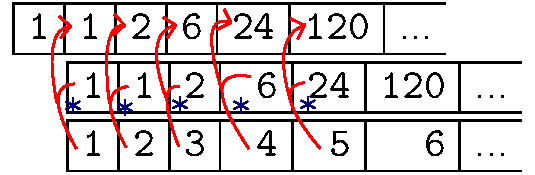
\includegraphics[width=8.98858717040535cm,height=2.94680571953299cm]{functional-lecture07-via-latex-2.pdf}}
\end{itemize}

\section{Power series and differential equations}

\begin{itemize}
  \item Differential equations idea due to Henning Thielemann.
  {\small{{\tmstrong{Just an example.}}}}
  
  \item Expression $P (x) = \sum_{i = 0}^n a_i x^i$ defines a polynomial for
  $n < \infty$ and a power series for $n = \infty$.
  
  \item If we define
  
  {\hlkwa{let rec }}{\hlstd{lfold{\textunderscore}right f l base
  }}{\hlopt{=}}{\hlendline{}}\\
  {\hlstd{ \ }}{\hlkwa{match }}{\hlstd{l }}{\hlkwa{with}}{\hlendline{}}\\
  {\hlstd{ \ \ \ }}{\hlopt{\textbar }}{\hlkwd{LNil }}{\hlopt{->
  }}{\hlstd{base{\hlendline{}}\\
  \ \ \ }}{\hlopt{\textbar }}{\hlkwd{LCons }}{\hlopt{(}}{\hlstd{a}}{\hlopt{,
  }}{\hlkwa{lazy }}{\hlstd{l}}{\hlopt{) -> }}{\hlstd{f a
  }}{\hlopt{(}}{\hlstd{lfold{\textunderscore}right f l
  base}}{\hlopt{)}}{\hlendline{}}
  
  then we can compute polynomials
  
  {\hlkwa{let }}{\hlstd{horner x l }}{\hlopt{=}}{\hlendline{}}\\
  {\hlstd{ \ lfold{\textunderscore}right }}{\hlopt{(}}{\hlkwa{fun }}{\hlstd{c
  sum }}{\hlopt{-> }}{\hlstd{c }}{\hlopt{+. }}{\hlstd{x }}{\hlopt{*.
  }}{\hlstd{sum}}{\hlopt{) }}{\hlstd{l }}{\hlnum{0}}{\hlopt{.}}{\hlendline{}}
  
  \item But it will not work for infinite power series!
  \begin{itemize}
    \item Does it make sense to compute the value at $x$ of a power series?
    
    \item Does it make sense to fold an infinite list?
  \end{itemize}
  \item If the power series converges for $x > 1$, then when the elements
  $a_n$ get small, the remaining sum $\sum_{i = n}^{\infty} a_i x^i$ is also
  small.
  
  \item \tmverbatim{lfold\_right} falls into an infinite loop on infinite
  lists. We need call-by-name / call-by-need semantics for the argument
  function \tmverbatim{f}.
  
  {\hlkwa{let rec }}{\hlstd{lazy{\textunderscore}foldr f l base
  }}{\hlopt{=}}{\hlendline{}}\\
  {\hlstd{ \ }}{\hlkwa{match }}{\hlstd{l }}{\hlkwa{with}}{\hlendline{}}\\
  {\hlstd{ \ \ \ }}{\hlopt{\textbar }}{\hlkwd{LNil }}{\hlopt{->
  }}{\hlstd{base{\hlendline{}}\\
  \ \ \ }}{\hlopt{\textbar }}{\hlkwd{LCons }}{\hlopt{(}}{\hlstd{a}}{\hlopt{,
  }}{\hlstd{ll}}{\hlopt{) ->}}{\hlendline{}}\\
  {\hlstd{ \ \ \ \ \ f a }}{\hlopt{(}}{\hlkwa{lazy
  }}{\hlopt{(}}{\hlstd{lazy{\textunderscore}foldr f
  }}{\hlopt{(}}{\hlkwc{Lazy}}{\hlopt{.}}{\hlstd{force ll}}{\hlopt{)
  }}{\hlstd{base}}{\hlopt{))}}{\hlendline{}}
  
  \item We need a stopping condition in the Horner algorithm step:
  
  {\hlkwa{let }}{\hlstd{lhorner x l }}{\hlopt{=}}{\hlendline{This is a bit of
  a hack,}}\\
  {\hlstd{ \ }}{\hlkwa{let }}{\hlstd{upd c sum }}{\hlopt{=}}{\hlendline{we
  hope to ``hit'' the interval $(0, \varepsilon]$.}}\\
  {\hlstd{ \ \ \ }}{\hlkwa{if }}{\hlstd{c }}{\hlopt{= }}{\hlnum{0}}{\hlopt{.
  }}{\hlstd{{\hlopt{\textbar\textbar}} }}{\hlstd{abs{\textunderscore}float c
  }}{\hlopt{> }}{\hlstd{epsilon{\textunderscore}float{\hlendline{}}\\
  \ \ \ }}{\hlkwa{then }}{\hlstd{c }}{\hlopt{+. }}{\hlstd{x }}{\hlopt{*.
  }}{\hlkwc{Lazy}}{\hlopt{.}}{\hlstd{force sum{\hlendline{}}\\
  \ \ \ }}{\hlkwa{else }}{\hlnum{0}}{\hlopt{. }}{\hlkwa{in}}{\hlendline{}}\\
  {\hlstd{ \ lazy{\textunderscore}foldr upd l
  }}{\hlnum{0}}{\hlopt{.}}{\hlendline{}}
  
  {\hlkwa{let }}{\hlstd{inv{\textunderscore}fact }}{\hlopt{= }}{\hlstd{lmap
  }}{\hlopt{(}}{\hlkwa{fun }}{\hlstd{n }}{\hlopt{-> }}{\hlnum{1}}{\hlopt{. /.
  }}{\hlstd{float{\textunderscore}of{\textunderscore}int n}}{\hlopt{)
  }}{\hlstd{lfact}}{\hlendline{}}\\
  {\hlkwa{let }}{\hlstd{e }}{\hlopt{= }}{\hlstd{lhorner }}{\hlnum{1}}{\hlopt{.
  }}{\hlstd{inv{\textunderscore}fact}}{\hlendline{}}
\end{itemize}

\subsection{Power series / polynomial operations}

{\small{\begin{itemize}
  \item {\hlkwa{let rec }}{\hlstd{add xs ys }}{\hlopt{=}}{\hlendline{}}\\
  {\hlstd{ \ }}{\hlkwa{match }}{\hlstd{xs}}{\hlopt{, }}{\hlstd{ys
  }}{\hlkwa{with}}{\hlendline{}}\\
  {\hlstd{ \ \ \ }}{\hlopt{\textbar }}{\hlkwd{LNil}}{\hlopt{,
  }}{\hlstd{{\textunderscore} }}{\hlopt{-> }}{\hlstd{ys{\hlendline{}}\\
  \ \ \ {\hlopt{\textbar}} {\textunderscore}}}{\hlopt{, }}{\hlkwd{LNil
  }}{\hlopt{-> }}{\hlstd{xs{\hlendline{}}\\
  \ \ \ }}{\hlopt{\textbar }}{\hlkwd{LCons
  }}{\hlopt{(}}{\hlstd{x}}{\hlopt{,}}{\hlstd{xs}}{\hlopt{), }}{\hlkwd{LCons
  }}{\hlopt{(}}{\hlstd{y}}{\hlopt{,}}{\hlstd{ys}}{\hlopt{)
  ->}}{\hlendline{}}\\
  {\hlstd{ \ \ \ \ \ }}{\hlkwd{LCons }}{\hlopt{(}}{\hlstd{x }}{\hlopt{+.
  }}{\hlstd{y}}{\hlopt{, }}{\hlkwa{lazy }}{\hlopt{(}}{\hlstd{add
  }}{\hlopt{(}}{\hlkwc{Lazy}}{\hlopt{.}}{\hlstd{force xs}}{\hlopt{)
  (}}{\hlkwc{Lazy}}{\hlopt{.}}{\hlstd{force ys}}{\hlopt{)))}}{\hlendline{}}
  
  \item {\hlkwa{let rec }}{\hlstd{sub xs ys }}{\hlopt{=}}{\hlendline{}}\\
  {\hlstd{ \ }}{\hlkwa{match }}{\hlstd{xs}}{\hlopt{, }}{\hlstd{ys
  }}{\hlkwa{with}}{\hlendline{}}\\
  {\hlstd{ \ \ \ }}{\hlopt{\textbar }}{\hlkwd{LNil}}{\hlopt{,
  }}{\hlstd{{\textunderscore} }}{\hlopt{-> }}{\hlstd{lmap
  }}{\hlopt{(}}{\hlkwa{fun }}{\hlstd{x}}{\hlopt{->
  }}{\hlstd{$\sim$}}{\hlopt{-.}}{\hlstd{x}}{\hlopt{)
  }}{\hlstd{ys{\hlendline{}}\\
  \ \ \ {\hlopt{\textbar}} {\textunderscore}}}{\hlopt{, }}{\hlkwd{LNil
  }}{\hlopt{-> }}{\hlstd{xs{\hlendline{}}\\
  \ \ \ }}{\hlopt{\textbar }}{\hlkwd{LCons
  }}{\hlopt{(}}{\hlstd{x}}{\hlopt{,}}{\hlstd{xs}}{\hlopt{), }}{\hlkwd{LCons
  }}{\hlopt{(}}{\hlstd{y}}{\hlopt{,}}{\hlstd{ys}}{\hlopt{)
  ->}}{\hlendline{}}\\
  {\hlstd{ \ \ \ \ \ }}{\hlkwd{LCons
  }}{\hlopt{(}}{\hlstd{x}}{\hlopt{-.}}{\hlstd{y}}{\hlopt{, }}{\hlkwa{lazy
  }}{\hlopt{(}}{\hlstd{add }}{\hlopt{(}}{\hlkwc{Lazy}}{\hlopt{.}}{\hlstd{force
  xs}}{\hlopt{) (}}{\hlkwc{Lazy}}{\hlopt{.}}{\hlstd{force
  ys}}{\hlopt{)))}}{\hlendline{}}
  
  \item {\hlkwa{let }}{\hlstd{scale s }}{\hlopt{= }}{\hlstd{lmap
  }}{\hlopt{(}}{\hlkwa{fun
  }}{\hlstd{x}}{\hlopt{->}}{\hlstd{s}}{\hlopt{*.}}{\hlstd{x}}{\hlopt{)}}{\hlendline{}}
  
  \item {\hlkwa{let rec }}{\hlstd{shift n xs }}{\hlopt{=}}{\hlendline{}}\\
  {\hlstd{ \ }}{\hlkwa{if }}{\hlstd{n }}{\hlopt{= }}{\hlnum{0 }}{\hlkwa{then
  }}{\hlstd{xs{\hlendline{}}\\
  \ }}{\hlkwa{else if }}{\hlstd{n }}{\hlopt{> }}{\hlnum{0 }}{\hlkwa{then
  }}{\hlkwd{LCons }}{\hlopt{(}}{\hlnum{0}}{\hlopt{. , }}{\hlkwa{lazy
  }}{\hlopt{(}}{\hlstd{shift
  }}{\hlopt{(}}{\hlstd{n}}{\hlopt{-}}{\hlnum{1}}{\hlopt{)
  }}{\hlstd{xs}}{\hlopt{))}}{\hlendline{}}\\
  {\hlstd{ \ }}{\hlkwa{else match }}{\hlstd{xs
  }}{\hlkwa{with}}{\hlendline{}}\\
  {\hlstd{ \ \ \ }}{\hlopt{\textbar }}{\hlkwd{LNil }}{\hlopt{->
  }}{\hlkwd{LNil}}{\hlendline{}}\\
  {\hlstd{ \ \ \ }}{\hlopt{\textbar }}{\hlkwd{LCons
  }}{\hlopt{(}}{\hlnum{0}}{\hlopt{., }}{\hlkwa{lazy }}{\hlstd{xs}}{\hlopt{) ->
  }}{\hlstd{shift }}{\hlopt{(}}{\hlstd{n}}{\hlopt{+}}{\hlnum{1}}{\hlopt{)
  }}{\hlstd{xs{\hlendline{}}\\
  \ \ \ {\hlopt{\textbar}} {\textunderscore} }}{\hlopt{-> }}{\hlstd{failwith
  }}{\hlstr{"shift: fractional division"}}{\hlendline{}}
  
  \item {\hlkwa{let rec }}{\hlstd{mul xs }}{\hlopt{=
  }}{\hlkwa{function}}{\hlendline{}}\\
  {\hlstd{ \ }}{\hlopt{\textbar }}{\hlkwd{LNil }}{\hlopt{->
  }}{\hlkwd{LNil}}{\hlendline{}}\\
  {\hlstd{ \ }}{\hlopt{\textbar }}{\hlkwd{LCons
  }}{\hlopt{(}}{\hlstd{y}}{\hlopt{, }}{\hlstd{ys}}{\hlopt{)
  ->}}{\hlendline{}}\\
  {\hlstd{ \ \ \ add }}{\hlopt{(}}{\hlstd{scale y xs}}{\hlopt{)
  (}}{\hlkwd{LCons }}{\hlopt{(}}{\hlnum{0}}{\hlopt{., }}{\hlkwa{lazy
  }}{\hlopt{(}}{\hlstd{mul xs
  }}{\hlopt{(}}{\hlkwc{Lazy}}{\hlopt{.}}{\hlstd{force
  ys}}{\hlopt{))))}}{\hlendline{}}
  
  \item {\hlkwa{let rec }}{\hlstd{div xs ys }}{\hlopt{=}}{\hlendline{}}\\
  {\hlstd{ \ }}{\hlkwa{match }}{\hlstd{xs}}{\hlopt{, }}{\hlstd{ys
  }}{\hlkwa{with}}{\hlendline{}}\\
  {\hlstd{ \ }}{\hlopt{\textbar }}{\hlkwd{LNil}}{\hlopt{,
  }}{\hlstd{{\textunderscore} }}{\hlopt{-> }}{\hlkwd{LNil}}{\hlendline{}}\\
  {\hlstd{ \ }}{\hlopt{\textbar }}{\hlkwd{LCons
  }}{\hlopt{(}}{\hlnum{0}}{\hlopt{., }}{\hlstd{xs'}}{\hlopt{), }}{\hlkwd{LCons
  }}{\hlopt{(}}{\hlnum{0}}{\hlopt{., }}{\hlstd{ys'}}{\hlopt{)
  ->}}{\hlendline{}}\\
  {\hlstd{ \ \ \ div }}{\hlopt{(}}{\hlkwc{Lazy}}{\hlopt{.}}{\hlstd{force
  xs'}}{\hlopt{) (}}{\hlkwc{Lazy}}{\hlopt{.}}{\hlstd{force
  ys'}}{\hlopt{)}}{\hlendline{}}\\
  {\hlstd{ \ }}{\hlopt{\textbar }}{\hlkwd{LCons
  }}{\hlopt{(}}{\hlstd{x}}{\hlopt{, }}{\hlstd{xs'}}{\hlopt{), }}{\hlkwd{LCons
  }}{\hlopt{(}}{\hlstd{y}}{\hlopt{, }}{\hlstd{ys'}}{\hlopt{)
  ->}}{\hlendline{}}\\
  {\hlstd{ \ \ \ }}{\hlkwa{let }}{\hlstd{q }}{\hlopt{= }}{\hlstd{x
  }}{\hlopt{/. }}{\hlstd{y }}{\hlkwa{in}}{\hlendline{}}\\
  {\hlstd{ \ \ \ }}{\hlkwd{LCons }}{\hlopt{(}}{\hlstd{q}}{\hlopt{,
  }}{\hlkwa{lazy }}{\hlopt{(}}{\hlstd{divSeries }}{\hlopt{(}}{\hlstd{sub
  }}{\hlopt{(}}{\hlkwc{Lazy}}{\hlopt{.}}{\hlstd{force
  xs'}}{\hlopt{)}}{\hlendline{}}\\
  {\hlstd{ \ \ \ \ \ \ \ \ \ \ \ \ \ \ \ \ \ \ \ \ \ \ \ \ \ \ \ \ \ \ \ \
  }}{\hlopt{(}}{\hlstd{scale q
  }}{\hlopt{(}}{\hlkwc{Lazy}}{\hlopt{.}}{\hlstd{force ys'}}{\hlopt{)))
  }}{\hlstd{ys}}{\hlopt{))}}{\hlendline{}}\\
  {\hlstd{ \ }}{\hlopt{\textbar }}{\hlkwd{LCons
  }}{\hlstd{{\textunderscore}}}{\hlopt{, }}{\hlkwd{LNil }}{\hlopt{->
  }}{\hlstd{failwith }}{\hlstr{"divSeries: division by zero"}}{\hlendline{}}
  
  \item {\hlkwa{let }}{\hlstd{integrate c xs }}{\hlopt{=}}{\hlendline{}}\\
  {\hlstd{ \ }}{\hlkwd{LCons }}{\hlopt{(}}{\hlstd{c}}{\hlopt{, }}{\hlkwa{lazy
  }}{\hlopt{(}}{\hlstd{lmap }}{\hlopt{(}}{\hlstd{uncurry }}{\hlopt{(/.))
  (}}{\hlstd{lzip }}{\hlopt{(}}{\hlstd{xs}}{\hlopt{,
  }}{\hlstd{posnums}}{\hlopt{))))}}{\hlendline{}}
  
  \item {\hlkwa{let }}{\hlstd{ltail }}{\hlopt{=
  }}{\hlkwa{function}}{\hlendline{}}\\
  {\hlstd{ \ }}{\hlopt{\textbar }}{\hlkwd{LNil }}{\hlopt{->
  }}{\hlstd{invalid{\textunderscore}arg
  }}{\hlstr{"ltail"}}{\hlstd{{\hlendline{}}\\
  \ }}{\hlopt{\textbar }}{\hlkwd{LCons
  }}{\hlopt{(}}{\hlstd{{\textunderscore}}}{\hlopt{, }}{\hlkwa{lazy
  }}{\hlstd{tl}}{\hlopt{) -> }}{\hlstd{tl}}{\hlendline{}}
  
  \item {\hlkwa{let }}{\hlstd{differentiate xs }}{\hlopt{=}}{\hlendline{}}\\
  {\hlstd{ \ lmap }}{\hlopt{(}}{\hlstd{uncurry }}{\hlopt{( *.))
  (}}{\hlstd{lzip }}{\hlopt{(}}{\hlstd{ltail xs}}{\hlopt{,
  }}{\hlstd{posnums}}{\hlopt{))}}{\hlendline{}}
\end{itemize}}}

\subsection{Differential equations}

\begin{itemize}
  \item $\frac{\mathd \sin x}{\mathd x} = \cos x, \frac{\mathd \cos x}{\mathd
  x} = - \sin x, \sin 0 = 0, \cos 0 = 1$.
  
  \item We will solve the corresponding integral equations. {\tmem{Why?}}
  
  \item We cannot define the integral by direct recursion like this:
  
  {\hlkwa{let rec }}{\hlstd{sin }}{\hlopt{= }}{\hlstd{integrate
  }}{\hlopt{(}}{\hlstd{of{\textunderscore}int }}{\hlnum{0}}{\hlopt{)
  }}{\hlstd{cos}}{\hlendline{Unary op. {\tiny{{\hlkwa{let
  }}{\hlopt{(}}{\hlstd{$\sim$}}{\hlopt{-:) =}}}}}}\\
  {\hlkwa{and }}{\hlstd{cos }}{\hlopt{= }}{\hlstd{integrate
  }}{\hlopt{(}}{\hlstd{of{\textunderscore}int }}{\hlnum{1}}{\hlopt{)
  }}{\hlstd{$\sim$}}{\hlopt{-:}}{\hlstd{sin}}{\hlendline{ {\tiny{{\hlstd{lmap
  }}{\hlopt{(}}{\hlkwa{fun }}{\hlstd{x}}{\hlopt{->
  }}{\hlstd{$\sim$}}{\hlopt{-.}}{\hlstd{x}}{\hlopt{)}}}}}}
  
  unfortunately fails:
  
  \tmverbatim{Error: This kind of expression is not allowed as right-hand side
  of `let rec'}
  \begin{itemize}
    \item Even changing the second argument of \tmverbatim{integrate} to
    call-by-need does not help, because OCaml cannot represent the values that
    \tmverbatim{x} and \tmverbatim{y} refer to.
  \end{itemize}
  \item We need to inline a bit of \tmverbatim{integrate} so that OCaml knows
  how to start building the recursive structure.
  
  {\hlkwa{let }}{\hlstd{integ xs }}{\hlopt{= }}{\hlstd{lmap
  }}{\hlopt{(}}{\hlstd{uncurry }}{\hlopt{(/.)) (}}{\hlstd{lzip
  }}{\hlopt{(}}{\hlstd{xs}}{\hlopt{,
  }}{\hlstd{posnums}}{\hlopt{))}}{\hlendline{}}\\
  {\hlkwa{let rec }}{\hlstd{sin }}{\hlopt{= }}{\hlkwd{LCons
  }}{\hlopt{(}}{\hlstd{of{\textunderscore}int }}{\hlnum{0}}{\hlopt{,
  }}{\hlkwa{lazy }}{\hlopt{(}}{\hlstd{integ cos}}{\hlopt{))}}{\hlendline{}}\\
  {\hlkwa{and }}{\hlstd{cos }}{\hlopt{= }}{\hlkwd{LCons
  }}{\hlopt{(}}{\hlstd{of{\textunderscore}int }}{\hlnum{1}}{\hlopt{,
  }}{\hlkwa{lazy }}{\hlopt{(}}{\hlstd{integ
  $\sim$}}{\hlopt{-:}}{\hlstd{sin}}{\hlopt{))}}{\hlendline{}}
  
  \item The complete example would look much more elegant in Haskell.
  
  \item Although this approach is not limited to linear equations, equations
  like Lotka-Volterra or Lorentz are not ``solvable'' -- computed coefficients
  quickly grow instead of quickly falling...
  
  \item Drawing functions are like in previous lecture, but with open curves.
  
  \item {\hlkwa{let }}{\hlstd{plot{\textunderscore}1D f $\sim$w $\sim$scale
  $\sim$t{\textunderscore}beg $\sim$t{\textunderscore}end
  }}{\hlopt{=}}{\hlendline{}}\\
  {\hlstd{ \ }}{\hlkwa{let }}{\hlstd{dt }}{\hlopt{=
  (}}{\hlstd{t{\textunderscore}end }}{\hlopt{-.
  }}{\hlstd{t{\textunderscore}beg}}{\hlopt{) /.
  }}{\hlstd{of{\textunderscore}int w }}{\hlkwa{in}}{\hlendline{}}\\
  {\hlstd{ \ }}{\hlkwc{Array}}{\hlopt{.}}{\hlstd{init w
  }}{\hlopt{(}}{\hlkwa{fun }}{\hlstd{i }}{\hlopt{->}}{\hlendline{}}\\
  {\hlstd{ \ \ \ }}{\hlkwa{let }}{\hlstd{y }}{\hlopt{= }}{\hlstd{lhorner
  }}{\hlopt{(}}{\hlstd{dt }}{\hlopt{*. }}{\hlstd{of{\textunderscore}int
  i}}{\hlopt{) }}{\hlstd{f }}{\hlkwa{in}}{\hlendline{}}\\
  {\hlstd{ \ \ \ i}}{\hlopt{, }}{\hlstd{to\_int }}{\hlopt{(}}{\hlstd{scale
  }}{\hlopt{*. }}{\hlstd{y}}{\hlopt{))}}{\hlendline{}}
\end{itemize}

\section{Arbitrary precision computation}

\begin{itemize}
  \item Putting it all together reveals drastic numerical errors for large
  $x$.
  
  {\hlkwa{let }}{\hlstd{graph }}{\hlopt{=}}{\hlendline{}}\\
  {\hlstd{ \ }}{\hlkwa{let }}{\hlstd{scale }}{\hlopt{=
  }}{\hlstd{of{\textunderscore}int h }}{\hlopt{/.
  }}{\hlstd{of{\textunderscore}int }}{\hlnum{8 }}{\hlkwa{in}}{\hlendline{}}\\
  {\hlstd{ \ }}{\hlopt{[}}{\hlstd{plot{\textunderscore}1D sin $\sim$w
  $\sim$h0}}{\hlopt{:(}}{\hlstd{h}}{\hlopt{/}}{\hlnum{2}}{\hlopt{)
  }}{\hlstd{$\sim$scale{\hlendline{}}\\
  \ \ \ \ \
  $\sim$t{\textunderscore}beg}}{\hlopt{:(}}{\hlstd{of{\textunderscore}int
  }}{\hlnum{0}}{\hlopt{)
  }}{\hlstd{$\sim$t{\textunderscore}end}}{\hlopt{:(}}{\hlstd{of{\textunderscore}int
  }}{\hlnum{15}}{\hlopt{),}}{\hlendline{}}\\
  {\hlstd{ \ \
  }}{\hlopt{(}}{\hlnum{250}}{\hlopt{,}}{\hlnum{250}}{\hlopt{,}}{\hlnum{0}}{\hlopt{);}}{\hlendline{}}\\
  {\hlstd{ \ \ plot{\textunderscore}1D cos $\sim$w
  $\sim$h0}}{\hlopt{:(}}{\hlstd{h}}{\hlopt{/}}{\hlnum{2}}{\hlopt{)
  }}{\hlstd{$\sim$scale{\hlendline{}}\\
  \ \ \ \
  $\sim$t{\textunderscore}beg}}{\hlopt{:(}}{\hlstd{of{\textunderscore}int
  }}{\hlnum{0}}{\hlopt{)
  }}{\hlstd{$\sim$t{\textunderscore}end}}{\hlopt{:(}}{\hlstd{of{\textunderscore}int
  }}{\hlnum{15}}{\hlopt{),}}{\hlendline{}}\\
  {\hlstd{ \ \
  }}{\hlopt{(}}{\hlnum{250}}{\hlopt{,}}{\hlnum{0}}{\hlopt{,}}{\hlnum{250}}{\hlopt{)]}}{\hlendline{}}\\
  {\hlkwa{let }}{\hlopt{() =
  }}{\hlstd{draw{\textunderscore}to{\textunderscore}screen $\sim$w $\sim$h
  graph}}{\hlendline{}}
  \begin{itemize}
    \item Floating-point numbers have limited precision.
    
    \item We break out of Horner method computations too quickly.
  \end{itemize}
  \scalebox{0.6}{\includegraphics{functional-lecture07-via-latex-3.pdf}}
  
  \item For infinite precision on rational numbers we use the
  \tmverbatim{nums} library.
  \begin{itemize}
    \item It does not help -- yet.
  \end{itemize}
  \item Generate a sequence of approximations to the power series limit at
  $x$.
  
  {\hlkwa{let }}{\hlstd{infhorner x l }}{\hlopt{=}}{\hlendline{}}\\
  {\hlstd{ \ }}{\hlkwa{let }}{\hlstd{upd c sum }}{\hlopt{=}}{\hlendline{}}\\
  {\hlstd{ \ \ \ }}{\hlkwd{LCons }}{\hlopt{(}}{\hlstd{c}}{\hlopt{,
  }}{\hlkwa{lazy }}{\hlopt{(}}{\hlstd{lmap }}{\hlopt{(}}{\hlkwa{fun
  }}{\hlstd{apx }}{\hlopt{->
  }}{\hlstd{c}}{\hlopt{+.}}{\hlstd{x}}{\hlopt{*.}}{\hlstd{apx}}{\hlopt{)}}{\hlendline{}}\\
  {\hlstd{ \ \ \ \ \ \ \ \ \ \ \ \ \ \ \ \ \ \ \ \ \
  }}{\hlopt{(}}{\hlkwc{Lazy}}{\hlopt{.}}{\hlstd{force sum}}{\hlopt{)))
  }}{\hlkwa{in}}{\hlendline{}}\\
  {\hlstd{ \ lazy{\textunderscore}foldr upd l }}{\hlopt{(}}{\hlkwd{LCons
  }}{\hlopt{(}}{\hlstd{of{\textunderscore}int }}{\hlnum{0}}{\hlopt{,
  }}{\hlkwa{lazy }}{\hlkwd{LNil}}{\hlopt{))}}{\hlendline{}}
  
  \item Find where the series converges -- as far as a given test is
  concerned.
  
  {\hlkwa{let rec }}{\hlstd{exact f }}{\hlopt{=
  }}{\hlkwa{function}}{\hlendline{We arbitrarily decide that convergence
  is}}\\
  {\hlstd{ \ }}{\hlopt{\textbar }}{\hlkwd{LNil }}{\hlopt{-> }}{\hlkwa{assert
  false}}{\hlendline{when three consecutive results are the same.}}\\
  {\hlstd{ \ }}{\hlopt{\textbar }}{\hlkwd{LCons
  }}{\hlopt{(}}{\hlstd{x0}}{\hlopt{, }}{\hlkwa{lazy }}{\hlopt{(}}{\hlkwd{LCons
  }}{\hlopt{(}}{\hlstd{x1}}{\hlopt{, }}{\hlkwa{lazy }}{\hlopt{(}}{\hlkwd{LCons
  }}{\hlopt{(}}{\hlstd{x2}}{\hlopt{,
  }}{\hlstd{{\textunderscore}}}{\hlopt{)))))}}{\hlendline{}}\\
  {\hlstd{ \ \ \ \ \ }}{\hlkwa{when }}{\hlstd{f x0 }}{\hlopt{= }}{\hlstd{f x1
  }}{\hlopt{\&\& }}{\hlstd{f x0 }}{\hlopt{= }}{\hlstd{f x2 }}{\hlopt{->
  }}{\hlstd{f x0{\hlendline{}}\\
  \ }}{\hlopt{\textbar }}{\hlkwd{LCons
  }}{\hlopt{(}}{\hlstd{{\textunderscore}}}{\hlopt{, }}{\hlkwa{lazy
  }}{\hlstd{tl}}{\hlopt{) -> }}{\hlstd{exact f tl}}{\hlendline{}}
  
  \item Draw the pixels of the graph at exact coordinates.
  
  {\hlkwa{let }}{\hlstd{plot{\textunderscore}1D f $\sim$w $\sim$h0 $\sim$scale
  $\sim$t{\textunderscore}beg $\sim$t{\textunderscore}end
  }}{\hlopt{=}}{\hlendline{}}\\
  {\hlstd{ \ }}{\hlkwa{let }}{\hlstd{dt }}{\hlopt{=
  (}}{\hlstd{t{\textunderscore}end }}{\hlopt{-.
  }}{\hlstd{t{\textunderscore}beg}}{\hlopt{) /.
  }}{\hlstd{of{\textunderscore}int w }}{\hlkwa{in}}{\hlendline{}}\\
  {\hlstd{ \ }}{\hlkwa{let }}{\hlstd{eval }}{\hlopt{= }}{\hlstd{exact
  }}{\hlopt{(}}{\hlkwa{fun }}{\hlstd{y}}{\hlopt{->
  }}{\hlstd{to{\textunderscore}int }}{\hlopt{(}}{\hlstd{scale }}{\hlopt{*.
  }}{\hlstd{y}}{\hlopt{)) }}{\hlkwa{in}}{\hlendline{}}\\
  {\hlstd{ \ }}{\hlkwc{Array}}{\hlopt{.}}{\hlstd{init w
  }}{\hlopt{(}}{\hlkwa{fun }}{\hlstd{i }}{\hlopt{->}}{\hlendline{}}\\
  {\hlstd{ \ \ \ }}{\hlkwa{let }}{\hlstd{y }}{\hlopt{= }}{\hlstd{infhorner
  }}{\hlopt{(}}{\hlstd{t{\textunderscore}beg }}{\hlopt{+. }}{\hlstd{dt
  }}{\hlopt{*. }}{\hlstd{of{\textunderscore}int i}}{\hlopt{) }}{\hlstd{f
  }}{\hlkwa{in}}{\hlendline{}}\\
  {\hlstd{ \ \ \ i}}{\hlopt{, }}{\hlstd{h0 }}{\hlopt{+ }}{\hlstd{eval
  y}}{\hlopt{)}}{\hlendline{}}
  
  \item Success! If a power series had every third term contributing we would
  have to check three terms in the function \tmverbatim{exact}...
  \begin{itemize}
    \item We could like in \tmverbatim{lhorner} test for \tmverbatim{f x0 = f
    x1 \&\& not x0 =. x1}
  \end{itemize}
  \item Example \tmverbatim{n\_chain}: nuclear chain reaction--{\tmem{A decays
  into B decays into C}}
  \begin{itemize}
    \item
    {\small{\href{http://en.wikipedia.org/wiki/Radioactive_decay#Chain-decay_processes}{http://en.wikipedia.org/wiki/Radioactive\_decay\#Chain-decay\_processes}}}
  \end{itemize}
  {\small{{\hlkwa{let }}{\hlstd{n{\textunderscore}chain $\sim$nA0 $\sim$nB0
  $\sim$lA $\sim$lB }}{\hlopt{=}}{\hlendline{}}\\
  {\hlstd{ \ }}{\hlkwa{let rec }}{\hlstd{nA }}{\hlopt{=}}{\hlendline{}}\\
  {\hlstd{ \ \ \ }}{\hlkwd{LCons }}{\hlopt{(}}{\hlstd{nA0}}{\hlopt{,
  }}{\hlkwa{lazy }}{\hlopt{(}}{\hlstd{integ
  }}{\hlopt{(}}{\hlstd{$\sim$}}{\hlopt{-.}}{\hlstd{lA }}{\hlopt{*:.
  }}{\hlstd{nA}}{\hlopt{)))}}{\hlendline{}}\\
  {\hlstd{ \ }}{\hlkwa{and }}{\hlstd{nB }}{\hlopt{=}}{\hlendline{}}\\
  {\hlstd{ \ \ \ }}{\hlkwd{LCons }}{\hlopt{(}}{\hlstd{nB0}}{\hlopt{,
  }}{\hlkwa{lazy }}{\hlopt{(}}{\hlstd{integ
  }}{\hlopt{(}}{\hlstd{$\sim$}}{\hlopt{-.}}{\hlstd{lB }}{\hlopt{*:.
  }}{\hlstd{nB }}{\hlopt{+: }}{\hlstd{lA }}{\hlopt{*:.
  }}{\hlstd{nA}}{\hlopt{))) }}{\hlkwa{in}}{\hlendline{}}\\
  {\hlstd{ \ nA}}{\hlopt{, }}{\hlstd{nB}}{\hlendline{}}}}
\end{itemize}
\scalebox{0.6}{\includegraphics{functional-lecture07-via-latex-4.pdf}}

\section{Circular data structures: double-linked list}

\begin{itemize}
  \item Without delayed computation, the ability to define data structures
  with referential cycles is very limited.
  
  \item Double-linked lists contain such cycles between any two nodes even if
  they are not cyclic when following only {\tmem{forward}} or
  {\tmem{backward}} links.
  
  \raisebox{-0.355447230476445\height}{\includegraphics[width=18.705365341729cm,height=0.98225764134855cm]{functional-lecture07-via-latex-5.pdf}}
  
  \item We need to ``break'' the cycles by making some links lazy.
  
  \item {\hlkwa{type }}{\hlstd{'a dllist }}{\hlopt{=}}{\hlendline{}}\\
  {\hlstd{ \ }}{\hlkwd{DLNil }}{\hlopt{\textbar }}{\hlkwd{DLCons }}{\hlkwa{of
  }}{\hlstd{'a dllist }}{\hlkwc{Lazy}}{\hlopt{.}}{\hlstd{t }}{\hlopt{*
  }}{\hlstd{'a }}{\hlopt{* }}{\hlstd{'a dllist}}{\hlendline{}}
  
  \item {\hlkwa{let rec }}{\hlstd{dldrop n l }}{\hlopt{=}}{\hlendline{}}\\
  {\hlstd{ \ }}{\hlkwa{match }}{\hlstd{l }}{\hlkwa{with}}{\hlendline{}}\\
  {\hlstd{ \ \ \ }}{\hlopt{\textbar }}{\hlkwd{DLCons
  }}{\hlopt{(}}{\hlstd{{\textunderscore}}}{\hlopt{, }}{\hlstd{x}}{\hlopt{,
  }}{\hlstd{xs}}{\hlopt{) }}{\hlkwa{when }}{\hlstd{n}}{\hlopt{>}}{\hlnum{0
  }}{\hlopt{->}}{\hlendline{}}\\
  {\hlstd{ \ \ \ \ \ dldrop
  }}{\hlopt{(}}{\hlstd{n}}{\hlopt{-}}{\hlnum{1}}{\hlopt{)
  }}{\hlstd{xs{\hlendline{}}\\
  \ \ \ {\hlopt{\textbar}} {\textunderscore} }}{\hlopt{->
  }}{\hlstd{l}}{\hlendline{}}
  
  \item {\hlkwa{let }}{\hlstd{dllist{\textunderscore}of{\textunderscore}list l
  }}{\hlopt{=}}{\hlendline{}}\\
  {\hlstd{ \ }}{\hlkwa{let rec }}{\hlstd{dllist prev l
  }}{\hlopt{=}}{\hlendline{}}\\
  {\hlstd{ \ \ \ }}{\hlkwa{match }}{\hlstd{l }}{\hlkwa{with}}{\hlendline{}}\\
  {\hlstd{ \ \ \ \ \ }}{\hlopt{\textbar  [] ->
  }}{\hlkwd{DLNil}}{\hlendline{}}\\
  {\hlstd{ \ \ \ \ \ {\hlopt{\textbar}} x}}{\hlopt{::}}{\hlstd{xs
  }}{\hlopt{->}}{\hlendline{}}\\
  {\hlstd{ \ \ \ \ \ \ \ }}{\hlkwa{let rec }}{\hlstd{cell
  }}{\hlopt{=}}{\hlendline{}}\\
  {\hlstd{ \ \ \ \ \ \ \ \ \ }}{\hlkwa{lazy }}{\hlopt{(}}{\hlkwd{DLCons
  }}{\hlopt{(}}{\hlstd{prev}}{\hlopt{, }}{\hlstd{x}}{\hlopt{, }}{\hlstd{dllist
  cell xs}}{\hlopt{)) }}{\hlkwa{in}}{\hlendline{}}\\
  {\hlstd{ \ \ \ \ \ \ \ }}{\hlkwc{Lazy}}{\hlopt{.}}{\hlstd{force cell
  }}{\hlkwa{in}}{\hlendline{}}\\
  {\hlstd{ \ dllist }}{\hlopt{(}}{\hlkwa{lazy }}{\hlkwd{DLNil}}{\hlopt{)
  }}{\hlstd{l}}{\hlendline{}}
  
  \item {\hlkwa{let rec }}{\hlstd{dltake n l }}{\hlopt{=}}{\hlendline{}}\\
  {\hlstd{ \ }}{\hlkwa{match }}{\hlstd{l }}{\hlkwa{with}}{\hlendline{}}\\
  {\hlstd{ \ \ \ }}{\hlopt{\textbar }}{\hlkwd{DLCons
  }}{\hlopt{(}}{\hlstd{{\textunderscore}}}{\hlopt{, }}{\hlstd{x}}{\hlopt{,
  }}{\hlstd{xs}}{\hlopt{) }}{\hlkwa{when }}{\hlstd{n}}{\hlopt{>}}{\hlnum{0
  }}{\hlopt{->}}{\hlendline{}}\\
  {\hlstd{ \ \ \ \ \ x}}{\hlopt{::}}{\hlstd{dltake
  }}{\hlopt{(}}{\hlstd{n}}{\hlopt{-}}{\hlnum{1}}{\hlopt{)
  }}{\hlstd{xs{\hlendline{}}\\
  \ \ \ {\hlopt{\textbar}} {\textunderscore} }}{\hlopt{-> []}}{\hlendline{}}
  
  \item {\hlkwa{let rec }}{\hlstd{dlbackwards n l
  }}{\hlopt{=}}{\hlendline{}}\\
  {\hlstd{ \ }}{\hlkwa{match }}{\hlstd{l }}{\hlkwa{with}}{\hlendline{}}\\
  {\hlstd{ \ \ \ }}{\hlopt{\textbar }}{\hlkwd{DLCons }}{\hlopt{(}}{\hlkwa{lazy
  }}{\hlstd{xs}}{\hlopt{, }}{\hlstd{x}}{\hlopt{,
  }}{\hlstd{{\textunderscore}}}{\hlopt{) }}{\hlkwa{when
  }}{\hlstd{n}}{\hlopt{>}}{\hlnum{0 }}{\hlopt{->}}{\hlendline{}}\\
  {\hlstd{ \ \ \ \ \ x}}{\hlopt{::}}{\hlstd{dlbackwards
  }}{\hlopt{(}}{\hlstd{n}}{\hlopt{-}}{\hlnum{1}}{\hlopt{)
  }}{\hlstd{xs{\hlendline{}}\\
  \ \ \ {\hlopt{\textbar}} {\textunderscore} }}{\hlopt{-> []}}{\hlendline{}}
\end{itemize}

\section{Input-Output streams}

\begin{itemize}
  \item The stream type used a throwaway argument to make a suspension
  
  {\hlkwa{type }}{\hlstd{'a stream }}{\hlopt{= }}{\hlkwd{SNil
  }}{\hlopt{\textbar }}{\hlkwd{SCons }}{\hlkwa{of }}{\hlstd{'a }}{\hlopt{*
  (}}{\hlkwb{unit }}{\hlopt{-> }}{\hlstd{'a stream}}{\hlopt{)}}{\hlendline{}}
  
  What if we take a real argument?
  
  {\hlkwa{type }}{\hlopt{(}}{\hlstd{'a}}{\hlopt{, }}{\hlstd{'b}}{\hlopt{)
  }}{\hlstd{iostream }}{\hlopt{=}}{\hlendline{}}\\
  {\hlstd{ \ }}{\hlkwd{EOS }}{\hlopt{\textbar }}{\hlkwd{More }}{\hlkwa{of
  }}{\hlstd{'b }}{\hlopt{* (}}{\hlstd{'a }}{\hlopt{-> (}}{\hlstd{'a}}{\hlopt{,
  }}{\hlstd{'b}}{\hlopt{) }}{\hlstd{iostream}}{\hlopt{)}}{\hlendline{}}
  
  A stream that for a single input value produces an output value.
  
  \item {\hlkwa{type }}{\hlstd{'a istream }}{\hlopt{=
  (}}{\hlkwb{unit}}{\hlopt{, }}{\hlstd{'a}}{\hlopt{)
  }}{\hlstd{iostream}}{\hlendline{}}\\
  Input stream produces output when ``asked''.
  
  {\hlkwa{type }}{\hlstd{'a ostream }}{\hlopt{= (}}{\hlstd{'a}}{\hlopt{,
  }}{\hlkwb{unit}}{\hlopt{) }}{\hlstd{iostream}}{\hlendline{}}\\
  Output stream consumes provided input.
  \begin{itemize}
    \item Sorry, the confusion arises from adapting the {\tmem{input file /
    output file}} terminology, also used for streams.
  \end{itemize}
  \item We can compose streams: directing output of one to input of another.
  
  {\hlkwa{let rec }}{\hlstd{compose sf sg }}{\hlopt{=}}{\hlendline{}}\\
  {\hlstd{ \ }}{\hlkwa{match }}{\hlstd{sg }}{\hlkwa{with}}{\hlendline{}}\\
  {\hlstd{ \ }}{\hlopt{\textbar }}{\hlkwd{EOS }}{\hlopt{->
  }}{\hlkwd{EOS}}{\hlendline{No more output.}}\tmverbatim{\\
  \ }{\hlopt{\textbar }}{\hlkwd{More }}{\hlopt{(}}{\hlstd{z}}{\hlopt{,
  }}{\hlstd{g}}{\hlopt{) ->}}{\hlendline{}}\\
  {\hlstd{ \ \ \ }}{\hlkwa{match }}{\hlstd{sf }}{\hlkwa{with}}{\hlendline{No
  more}}\\
  {\hlstd{ \ \ \ }}{\hlopt{\textbar }}{\hlkwd{EOS }}{\hlopt{-> }}{\hlkwd{More
  }}{\hlopt{(}}{\hlstd{z}}{\hlopt{, }}{\hlkwa{fun }}{\hlstd{{\textunderscore}
  }}{\hlopt{-> }}{\hlkwd{EOS}}{\hlopt{)}}{\hlendline{input ``processing
  power''.}}\\
  \ \ \ {\hlopt{\textbar }}{\hlkwd{More }}{\hlopt{(}}{\hlstd{y}}{\hlopt{,
  }}{\hlstd{f}}{\hlopt{) ->}}{\hlendline{}}\\
  {\hlstd{ \ \ \ \ \ }}{\hlkwa{let }}{\hlstd{update x }}{\hlopt{=
  }}{\hlstd{compose }}{\hlopt{(}}{\hlstd{f x}}{\hlopt{) (}}{\hlstd{g
  y}}{\hlopt{) }}{\hlkwa{in}}{\hlendline{}}\\
  {\hlstd{ \ \ \ \ \ }}{\hlkwd{More }}{\hlopt{(}}{\hlstd{z}}{\hlopt{,
  }}{\hlstd{update}}{\hlopt{)}}{\hlendline{}}
  \begin{itemize}
    \item Every box has one incoming and one outgoing
    wire:\raisebox{-0.465822087168946\height}{\includegraphics[width=1.32090384363112cm,height=4.40338449429358cm]{functional-lecture07-via-latex-6.pdf}}
    
    \item Notice how the output stream is ahead of the input stream.
  \end{itemize}
\end{itemize}

\subsection{Pipes}

\begin{itemize}
  \item We need a more flexible input-output stream definition.
  \begin{itemize}
    \item Consume several inputs to produce a single output.
    
    \item Produce several outputs after a single input (or even without
    input).
    
    \item No need for a dummy when producing output requires input.
  \end{itemize}
  \item After Haskell, we call the data structure \tmverbatim{pipe}.
  
  {\hlkwa{type }}{\hlopt{(}}{\hlstd{'a}}{\hlopt{, }}{\hlstd{'b}}{\hlopt{)
  }}{\hlstd{pipe }}{\hlopt{=}}{\hlendline{}}\\
  {\hlstd{ \ }}{\hlkwd{EOP}}{\hlendline{}}\\
  {\hlopt{\textbar }}{\hlkwd{Yield }}{\hlkwa{of }}{\hlstd{'b }}{\hlopt{*
  (}}{\hlstd{'a}}{\hlopt{, }}{\hlstd{'b}}{\hlopt{)
  }}\tmverbatim{pipe}{\hlendline{For incremental streams change to
  lazy.}}\tmverbatim{\\
  {\hlopt{\textbar}} }{\hlkwd{Await }}{\hlkwa{of }}{\hlstd{'a }}{\hlopt{->
  (}}{\hlstd{'a}}{\hlopt{, }}{\hlstd{'b}}{\hlopt{)
  }}{\hlstd{pipe}}{\hlendline{}}
  
  \item Again, we can have producing output only {\tmem{input pipes}} and
  consuming input only {\tmem{output pipes}}.
  
  {\hlkwa{type }}{\hlstd{'a ipipe }}{\hlopt{= (}}{\hlkwb{unit}}{\hlopt{,
  }}{\hlstd{'a}}{\hlopt{) }}{\hlstd{pipe}}{\hlendline{}}\\
  {\hlkwa{type }}{\hlstd{void}}{\hlendline{}}\\
  {\hlkwa{type }}{\hlstd{'a opipe }}{\hlopt{= (}}{\hlstd{'a}}{\hlopt{,
  }}{\hlstd{void}}{\hlopt{) }}{\hlstd{pipe}}{\hlendline{}}
  \begin{itemize}
    \item Why \tmverbatim{void} rather than \tmverbatim{unit}, and why only
    for \tmverbatim{opipe}?
  \end{itemize}
  \item Composition of pipes is like ``concatenating them in space'' or
  connecting boxes:
  
  {\hlkwa{let rec }}{\hlstd{compose pf pg }}{\hlopt{=}}{\hlendline{}}\\
  {\hlstd{ \ }}{\hlkwa{match }}{\hlstd{pg }}{\hlkwa{with}}{\hlendline{}}\\
  {\hlstd{ \ }}{\hlopt{\textbar }}{\hlkwd{EOP }}{\hlopt{->
  }}{\hlkwd{EOP}}{\hlendline{Done producing results.}}\\
  {\hlstd{ \ }}{\hlopt{\textbar }}{\hlkwd{Yield
  }}{\hlopt{(}}{\hlstd{z}}{\hlopt{, }}{\hlstd{pg'}}{\hlopt{) ->
  }}{\hlkwd{Yield }}{\hlopt{(}}{\hlstd{z}}{\hlopt{, }}{\hlstd{compose pf
  pg'}}{\hlopt{)}}{\hlendline{Ready result.}}\\
  {\hlstd{ \ }}{\hlopt{\textbar }}{\hlkwd{Await }}{\hlstd{g
  }}{\hlopt{->}}{\hlendline{}}\\
  {\hlstd{ \ \ \ }}{\hlkwa{match }}{\hlstd{pf }}{\hlkwa{with}}{\hlendline{}}\\
  {\hlstd{ \ \ \ }}{\hlopt{\textbar }}{\hlkwd{EOP }}{\hlopt{->
  }}{\hlkwd{EOP}}{\hlendline{End of input.}}\\
  {\hlstd{ \ \ \ }}{\hlopt{\textbar }}{\hlkwd{Yield
  }}{\hlopt{(}}{\hlstd{y}}{\hlopt{, }}{\hlstd{pf'}}{\hlopt{) ->
  }}{\hlstd{compose pf' }}{\hlopt{(}}{\hlstd{g
  y}}{\hlopt{)}}{\hlendline{Compute next result.}}\\
  {\hlstd{ \ \ \ }}{\hlopt{\textbar }}{\hlkwd{Await }}{\hlstd{f
  }}{\hlopt{->}}{\hlendline{}}\\
  {\hlstd{ \ \ \ \ \ }}{\hlkwa{let }}{\hlstd{update x }}{\hlopt{=
  }}{\hlstd{compose }}{\hlopt{(}}{\hlstd{f x}}{\hlopt{) }}{\hlstd{pg
  }}{\hlkwa{in}}{\hlendline{}}\\
  {\hlstd{ \ \ \ \ \ }}{\hlkwd{Await }}{\hlstd{update}}{\hlendline{Wait for
  more input.}}
  
  {\hlkwa{let }}{\hlopt{(>->) }}{\hlstd{pf pg }}{\hlopt{= }}{\hlstd{compose pf
  pg}}{\hlendline{}}
  
  \item Appending pipes means ``concatenating them in time'' or adding more
  fuel to a box:
  
  {\hlkwa{let rec }}{\hlstd{append pf pg }}{\hlopt{=}}{\hlendline{}}\\
  {\hlstd{ \ }}{\hlkwa{match }}{\hlstd{pf }}{\hlkwa{with}}{\hlendline{}}\\
  {\hlstd{ \ }}{\hlopt{\textbar }}{\hlkwd{EOP }}{\hlopt{->
  }}\tmverbatim{pg}{\hlendline{When \tmverbatim{pf} runs out, use
  \tmverbatim{pg}.}}\tmverbatim{\\
  \ {\hlopt{\textbar }}}{\hlkwd{Yield }}{\hlopt{(}}{\hlstd{z}}{\hlopt{,
  }}{\hlstd{pf'}}{\hlopt{) -> }}{\hlkwd{Yield
  }}{\hlopt{(}}{\hlstd{z}}{\hlopt{, }}{\hlstd{append pf'
  pg}}{\hlopt{)}}{\hlendline{}}\\
  {\hlstd{ \ }}{\hlopt{\textbar }}{\hlkwd{Await }}{\hlstd{f
  }}{\hlopt{->}}{\hlendline{If \tmverbatim{pf} awaits input, continue when it
  comes.}}\\
  {\hlstd{ \ \ \ }}{\hlkwa{let }}{\hlstd{update x }}{\hlopt{= }}{\hlstd{append
  }}{\hlopt{(}}{\hlstd{f x}}{\hlopt{) }}{\hlstd{pg
  }}{\hlkwa{in}}{\hlendline{}}\\
  {\hlstd{ \ \ \ }}{\hlkwd{Await }}{\hlstd{update}}{\hlendline{}}
  
  \item Append a list of ready results in front of a pipe.
  
  {\hlkwa{let rec }}{\hlstd{yield{\textunderscore}all l tail
  }}{\hlopt{=}}{\hlendline{}}\\
  {\hlstd{ \ }}{\hlkwa{match }}{\hlstd{l }}{\hlkwa{with}}{\hlendline{}}\\
  {\hlstd{ \ }}{\hlopt{\textbar  [] -> }}{\hlstd{tail{\hlendline{}}\\
  \ {\hlopt{\textbar}} x}}{\hlopt{::}}{\hlstd{xs }}{\hlopt{-> }}{\hlkwd{Yield
  }}{\hlopt{(}}{\hlstd{x}}{\hlopt{, }}{\hlstd{yield{\textunderscore}all xs
  tail}}{\hlopt{)}}{\hlendline{}}
  
  \item Iterate a pipe ({\tmstrong{not functional}}).
  
  {\hlkwa{let rec }}{\hlstd{iterate f }}{\hlopt{: }}{\hlstd{'a opipe
  }}{\hlopt{=}}{\hlendline{}}\\
  {\hlstd{ \ }}{\hlkwd{Await }}{\hlopt{(}}{\hlkwa{fun }}{\hlstd{x }}{\hlopt{->
  }}{\hlkwa{let }}{\hlopt{() = }}{\hlstd{f x }}{\hlkwa{in }}{\hlstd{iterate
  f}}{\hlopt{)}}{\hlendline{}}
\end{itemize}

\subsection{Example: pretty-printing}

\begin{itemize}
  \item Print hierarchically organized document with a limited line width.
  
  {\hlkwa{type }}{\hlstd{doc }}{\hlopt{=}}{\hlendline{}}\\
  {\hlstd{ \ }}{\hlkwd{Text }}{\hlkwa{of }}{\hlkwb{string }}{\hlopt{\textbar
  }}{\hlkwd{Line }}{\hlopt{\textbar }}{\hlkwd{Cat }}{\hlkwa{of }}{\hlstd{doc
  }}{\hlopt{* }}{\hlstd{doc {\hlopt{\textbar}} }}{\hlkwd{Group }}{\hlkwa{of
  }}{\hlstd{doc}}{\hlendline{}}
  
  \item {\hlkwa{let }}{\hlopt{(++) }}{\hlstd{d1 d2 }}{\hlopt{= }}{\hlkwd{Cat
  }}{\hlopt{(}}{\hlstd{d1}}{\hlopt{, }}{\hlkwd{Cat
  }}{\hlopt{(}}{\hlkwd{Line}}{\hlopt{,
  }}{\hlstd{d2}}{\hlopt{))}}{\hlendline{}}\\
  {\hlkwa{let }}{\hlopt{(!) }}{\hlstd{s }}{\hlopt{= }}{\hlkwd{Text
  }}{\hlstd{s}}{\hlendline{}}\\
  {\hlkwa{let }}{\hlstd{test{\textunderscore}doc }}{\hlopt{=}}{\hlendline{}}\\
  {\hlstd{ \ }}{\hlkwd{Group }}{\hlopt{(!}}{\hlstr{"Document"}}{\hlstd{
  }}{\hlopt{++}}{\hlendline{}}\\
  {\hlstd{ \ \ \ \ \ \ \ \ \ \ \ }}{\hlkwd{Group }}{\hlopt{(!}}{\hlstr{"First
  part"}}{\hlstd{ }}{\hlopt{++ !}}{\hlstr{"Second
  part"}}{\hlopt{))}}{\hlendline{}}
\end{itemize}
{\small{{\hlstd{\# }}{\hlkwa{let }}{\hlopt{() =
}}{\hlstd{print{\textunderscore}endline }}{\hlopt{(}}{\hlstd{pretty
}}{\hlnum{30 }}{\hlstd{test{\textunderscore}doc}}{\hlopt{);;}}{\hlendline{}}\\
{\hlkwd{Document}}{\hlendline{}}\\
{\hlkwd{First }}{\hlstd{part }}{\hlkwd{Second }}{\hlstd{part{\hlendline{}}\\
\# }}{\hlkwa{let }}{\hlopt{() = }}{\hlstd{print{\textunderscore}endline
}}{\hlopt{(}}{\hlstd{pretty }}{\hlnum{20
}}{\hlstd{test{\textunderscore}doc}}{\hlopt{);;}}{\hlendline{}}\\
{\hlkwd{Document}}{\hlendline{}}\\
{\hlkwd{First }}{\hlstd{part}}{\hlendline{}}\\
{\hlkwd{Second }}{\hlstd{part{\hlendline{}}\\
\# }}{\hlkwa{let }}{\hlopt{() = }}{\hlstd{print{\textunderscore}endline
}}{\hlopt{(}}{\hlstd{pretty }}{\hlnum{60
}}{\hlstd{test{\textunderscore}doc}}{\hlopt{);;}}{\hlendline{}}\\
{\hlkwd{Document First }}{\hlstd{part }}{\hlkwd{Second
}}{\hlstd{part}}{\hlendline{}}}}
\begin{itemize}
  \item Straightforward solution:
  
  {\hlkwa{let }}{\hlstd{pretty w d }}{\hlopt{=}}{\hlendline{Allowed width of
  line \tmverbatim{w}.}}\\
  {\hlstd{ \ }}{\hlkwa{let rec }}{\hlstd{width }}{\hlopt{=
  }}{\hlkwa{function}}{\hlendline{Total length of subdocument.}}\\
  {\hlstd{ \ \ \ }}{\hlopt{\textbar }}{\hlkwd{Text }}{\hlstd{z }}{\hlopt{->
  }}{\hlkwc{String}}{\hlopt{.}}{\hlstd{length z{\hlendline{}}\\
  \ \ \ }}{\hlopt{\textbar }}{\hlkwd{Line }}{\hlopt{->
  }}{\hlnum{1}}{\hlendline{}}\\
  {\hlstd{ \ \ \ }}{\hlopt{\textbar }}{\hlkwd{Cat
  }}{\hlopt{(}}{\hlstd{d1}}{\hlopt{, }}{\hlstd{d2}}{\hlopt{) ->
  }}{\hlstd{width d1 }}{\hlopt{+ }}{\hlstd{width d2{\hlendline{}}\\
  \ \ \ }}{\hlopt{\textbar }}{\hlkwd{Group }}{\hlstd{d }}{\hlopt{->
  }}{\hlstd{width d }}{\hlkwa{in}}{\hlendline{}}\\
  {\hlstd{ \ }}{\hlkwa{let rec }}{\hlstd{format f r }}{\hlopt{=
  }}{\hlkwa{function}}{\hlendline{Remaining space \tmverbatim{r}.}}\\
  {\hlstd{ \ \ \ }}{\hlopt{\textbar }}{\hlkwd{Text }}{\hlstd{z }}{\hlopt{->
  }}{\hlstd{z}}{\hlopt{, }}{\hlstd{r }}{\hlopt{-
  }}{\hlkwc{String}}{\hlopt{.}}{\hlstd{length z{\hlendline{}}\\
  \ \ \ }}{\hlopt{\textbar }}{\hlkwd{Line }}{\hlkwa{when }}{\hlstd{f
  }}{\hlopt{-> }}{\hlstr{" "}}{\hlopt{,
  }}{\hlstd{r}}{\hlopt{-}}{\hlnum{1}}{\hlendline{If \tmverbatim{not f} then
  line breaks.}}\\
  {\hlstd{ \ \ \ }}{\hlopt{\textbar }}{\hlkwd{Line }}{\hlopt{->
  }}{\hlstr{"}}{\hlesc{\textbackslash n}}{\hlstr{"}}{\hlopt{,
  }}{\hlstd{w{\hlendline{}}\\
  \ \ \ }}{\hlopt{\textbar }}{\hlkwd{Cat }}{\hlopt{(}}{\hlstd{d1}}{\hlopt{,
  }}{\hlstd{d2}}{\hlopt{) ->}}{\hlendline{}}\\
  {\hlstd{ \ \ \ \ \ }}{\hlkwa{let }}{\hlstd{s1}}{\hlopt{, }}{\hlstd{r
  }}{\hlopt{= }}{\hlstd{format f r d1 }}{\hlkwa{in}}{\hlendline{}}\\
  {\hlstd{ \ \ \ \ \ }}{\hlkwa{let }}{\hlstd{s2}}{\hlopt{, }}{\hlstd{r
  }}{\hlopt{= }}{\hlstd{format f r d2 }}{\hlkwa{in}}{\hlendline{}}\\
  {\hlstd{ \ \ \ \ \ s1 {\textasciicircum} s2}}{\hlopt{,
  }}\tmverbatim{r}{\hlendline{If following group fits, then without line
  breaks.}}\tmverbatim{\\
  \ \ \ }{\hlopt{\textbar }}{\hlkwd{Group }}{\hlstd{d }}{\hlopt{->
  }}{\hlstd{format }}{\hlopt{(}}{\hlstd{f {\hlopt{\textbar\textbar}} width d
  }}{\hlopt{<= }}{\hlstd{r}}{\hlopt{) }}{\hlstd{r d
  }}{\hlkwa{in}}{\hlendline{}}\\
  {\hlstd{ \ fst }}{\hlopt{(}}{\hlstd{format }}{\hlkwa{false }}{\hlstd{w
  d}}{\hlopt{)}}{\hlendline{}}
  
  \item Working with a stream of nodes.
  
  {\hlkwa{type }}{\hlopt{(}}{\hlstd{'a}}{\hlopt{, }}{\hlstd{'b}}{\hlopt{)
  }}{\hlstd{doc{\textunderscore}e }}{\hlopt{=}}{\hlendline{Annotated nodes,
  special for group beginning.}}\\
  {\hlstd{ \ }}{\hlkwd{TE }}{\hlkwa{of }}{\hlstd{'a }}{\hlopt{*
  }}{\hlkwb{string }}{\hlopt{\textbar }}{\hlkwd{LE }}{\hlkwa{of }}{\hlstd{'a
  {\hlopt{\textbar}} }}{\hlkwd{GBeg }}{\hlkwa{of }}{\hlstd{'b
  {\hlopt{\textbar}} }}{\hlkwd{GEnd }}{\hlkwa{of }}{\hlstd{'a}}{\hlendline{}}
  
  \item Normalize a subdocument -- remove empty groups.
  
  {\hlkwa{let rec }}{\hlstd{norm }}{\hlopt{=
  }}{\hlkwa{function}}{\hlendline{}}\\
  {\hlstd{ \ }}{\hlopt{\textbar }}{\hlkwd{Group }}{\hlstd{d }}{\hlopt{->
  }}{\hlstd{norm d{\hlendline{}}\\
  \ }}{\hlopt{\textbar }}{\hlkwd{Text }}{\hlstr{""}}{\hlstd{ }}{\hlopt{->
  }}{\hlkwd{None}}{\hlendline{}}\\
  {\hlstd{ \ }}{\hlopt{\textbar }}{\hlkwd{Cat }}{\hlopt{(}}{\hlkwd{Text
  }}{\hlstr{""}}{\hlopt{, }}{\hlstd{d}}{\hlopt{) -> }}{\hlstd{norm
  d{\hlendline{}}\\
  \ {\hlopt{\textbar}} d }}{\hlopt{-> }}{\hlkwd{Some
  }}{\hlstd{d}}{\hlendline{}}
  
  \item Generate the stream by infix traversal.
  
  {\hlkwa{let rec }}{\hlstd{gen }}{\hlopt{=
  }}{\hlkwa{function}}{\hlendline{}}\\
  {\hlstd{ \ }}{\hlopt{\textbar }}{\hlkwd{Text }}{\hlstd{z }}{\hlopt{->
  }}{\hlkwd{Yield }}{\hlopt{(}}{\hlkwd{TE
  }}{\hlopt{((),}}{\hlstd{z}}{\hlopt{),
  }}{\hlkwd{EOP}}{\hlopt{)}}{\hlendline{}}\\
  {\hlstd{ \ }}{\hlopt{\textbar }}{\hlkwd{Line }}{\hlopt{-> }}{\hlkwd{Yield
  }}{\hlopt{(}}{\hlkwd{LE }}{\hlopt{(),
  }}{\hlkwd{EOP}}{\hlopt{)}}{\hlendline{}}\\
  {\hlstd{ \ }}{\hlopt{\textbar }}{\hlkwd{Cat
  }}{\hlopt{(}}{\hlstd{d1}}{\hlopt{, }}{\hlstd{d2}}{\hlopt{) ->
  }}{\hlstd{append }}{\hlopt{(}}{\hlstd{gen d1}}{\hlopt{) (}}{\hlstd{gen
  d2}}{\hlopt{)}}{\hlendline{}}\\
  {\hlstd{ \ }}{\hlopt{\textbar }}{\hlkwd{Group }}{\hlstd{d
  }}{\hlopt{->}}{\hlendline{}}\\
  {\hlstd{ \ \ \ }}{\hlkwa{match }}{\hlstd{norm d
  }}{\hlkwa{with}}{\hlendline{}}\\
  {\hlstd{ \ \ \ }}{\hlopt{\textbar }}{\hlkwd{None }}{\hlopt{->
  }}{\hlkwd{EOP}}{\hlendline{}}\\
  {\hlstd{ \ \ \ }}{\hlopt{\textbar }}{\hlkwd{Some }}{\hlstd{d
  }}{\hlopt{->}}{\hlendline{}}\\
  {\hlstd{ \ \ \ \ \ }}{\hlkwd{Yield }}{\hlopt{(}}{\hlkwd{GBeg
  }}{\hlopt{(),}}{\hlendline{}}\\
  {\hlstd{ \ \ \ \ \ \ \ \ \ \ \ \ append }}{\hlopt{(}}{\hlstd{gen
  d}}{\hlopt{) (}}{\hlkwd{Yield }}{\hlopt{(}}{\hlkwd{GEnd }}{\hlopt{(),
  }}{\hlkwd{EOP}}{\hlopt{)))}}{\hlendline{}}
  
  \item Compute lengths of document prefixes, i.e. the position of each node
  counting by characters from the beginning of document.
  
  {\hlkwa{let rec }}{\hlstd{docpos curpos }}{\hlopt{=}}{\hlendline{}}\\
  {\hlstd{ \ }}{\hlkwd{Await }}{\hlopt{(}}{\hlkwa{function}}{\hlendline{We
  input from a \tmverbatim{doc\_e} pipe}}\\
  {\hlstd{ \ }}{\hlopt{\textbar }}{\hlkwd{TE
  }}{\hlopt{(}}{\hlstd{{\textunderscore}}}{\hlopt{, }}{\hlstd{z}}{\hlopt{)
  ->}}{\hlendline{}}\\
  {\hlstd{ \ \ \ }}{\hlkwd{Yield }}{\hlopt{(}}{\hlkwd{TE
  }}{\hlopt{(}}{\hlstd{curpos}}{\hlopt{,
  }}{\hlstd{z}}{\hlopt{),}}{\hlendline{and output \tmverbatim{doc\_e}
  annotated with position.}}\\
  {\hlstd{ \ \ \ \ \ \ \ \ \ \ docpos }}{\hlopt{(}}{\hlstd{curpos }}{\hlopt{+
  }}{\hlkwc{String}}{\hlopt{.}}{\hlstd{length z}}{\hlopt{))}}{\hlendline{}}\\
  {\hlstd{ \ }}{\hlopt{\textbar }}{\hlkwd{LE }}{\hlstd{{\textunderscore}
  }}{\hlopt{->}}{\hlendline{Spice and line breaks increase position by 1.}}\\
  {\hlstd{ \ \ \ }}{\hlkwd{Yield }}{\hlopt{(}}{\hlkwd{LE
  }}{\hlstd{curpos}}{\hlopt{, }}{\hlstd{docpos }}{\hlopt{(}}{\hlstd{curpos
  }}{\hlopt{+ }}{\hlnum{1}}{\hlopt{))}}{\hlendline{}}\\
  {\hlstd{ \ }}{\hlopt{\textbar }}{\hlkwd{GBeg }}{\hlstd{{\textunderscore}
  }}{\hlopt{->}}{\hlendline{Groups do not increase position.}}\\
  {\hlstd{ \ \ \ }}{\hlkwd{Yield }}{\hlopt{(}}{\hlkwd{GBeg
  }}{\hlstd{curpos}}{\hlopt{, }}{\hlstd{docpos
  curpos}}{\hlopt{)}}{\hlendline{}}\\
  {\hlstd{ \ }}{\hlopt{\textbar }}{\hlkwd{GEnd }}{\hlstd{{\textunderscore}
  }}{\hlopt{->}}{\hlendline{}}\\
  {\hlstd{ \ \ \ }}{\hlkwd{Yield }}{\hlopt{(}}{\hlkwd{GEnd
  }}{\hlstd{curpos}}{\hlopt{, }}{\hlstd{docpos
  curpos}}{\hlopt{))}}{\hlendline{}}{\hlstd{ \ }}
  
  {\hlkwa{let }}{\hlstd{docpos }}{\hlopt{= }}{\hlstd{docpos
  }}{\hlnum{0}}{\hlendline{The whole document starts at 0.}}
  
  \item Put the end position of the group into the group beginning marker, so
  that we can know whether to break it into multiple lines.
  
  {\hlkwa{let rec }}{\hlstd{grends grstack }}{\hlopt{=}}{\hlendline{}}\\
  {\hlstd{ \ }}{\hlkwd{Await }}{\hlopt{(}}{\hlkwa{function}}{\hlendline{}}\\
  {\hlstd{ \ }}{\hlopt{\textbar }}{\hlkwd{TE }}{\hlstd{{\textunderscore}
  {\hlopt{\textbar}} }}{\hlkwd{LE }}{\hlstd{{\textunderscore} }}{\hlkwa{as
  }}{\hlstd{e }}{\hlopt{->}}{\hlendline{}}\\
  {\hlstd{ \ \ \ }}{\hlopt{(}}{\hlkwa{match }}{\hlstd{grstack
  }}{\hlkwa{with}}{\hlendline{}}\\
  {\hlstd{ \ \ \ }}{\hlopt{\textbar  [] -> }}{\hlkwd{Yield
  }}{\hlopt{(}}{\hlstd{e}}{\hlopt{, }}{\hlstd{grends
  }}{\hlopt{[])}}{\hlendline{We can yield only when}}\\
  {\hlstd{ \ \ \ {\hlopt{\textbar}} gr}}{\hlopt{::}}{\hlstd{grs }}{\hlopt{->
  }}{\hlstd{grends
  }}{\hlopt{((}}{\hlstd{e}}{\hlopt{::}}{\hlstd{gr}}{\hlopt{)::}}{\hlstd{grs}}{\hlopt{))}}{\hlendline{no
  group is waiting.}}\\
  {\hlstd{ \ }}{\hlopt{\textbar }}{\hlkwd{GBeg }}{\hlstd{{\textunderscore}
  }}{\hlopt{-> }}{\hlstd{grends
  }}{\hlopt{([]::}}{\hlstd{grstack}}{\hlopt{)}}{\hlendline{Wait for end of
  group.}}\\
  {\hlstd{ \ }}{\hlopt{\textbar }}{\hlkwd{GEnd }}{\hlstd{endp
  }}{\hlopt{->}}{\hlendline{}}\\
  {\hlstd{ \ \ \ }}{\hlkwa{match }}{\hlstd{grstack
  }}{\hlkwa{with}}{\hlendline{End the group on top of stack.}}\\
  {\hlstd{ \ \ \ }}{\hlopt{\textbar  [] -> }}{\hlstd{failwith
  }}{\hlstr{"grends: unmatched group end marker"}}{\hlendline{}}\\
  {\hlstd{ \ \ \ }}{\hlopt{\textbar  [}}{\hlstd{gr}}{\hlopt{]
  ->}}{\hlendline{Top group -- we can yield now.}}\\
  {\hlstd{ \ \ \ \ \ yield{\textunderscore}all{\hlendline{}}\\
  \ \ \ \ \ \ \ }}{\hlopt{(}}{\hlkwd{GBeg
  }}{\hlstd{endp}}{\hlopt{::}}{\hlkwc{List}}{\hlopt{.}}{\hlstd{rev
  }}{\hlopt{(}}{\hlkwd{GEnd
  }}{\hlstd{endp}}{\hlopt{::}}{\hlstd{gr}}{\hlopt{))}}{\hlendline{}}\\
  {\hlstd{ \ \ \ \ \ \ \ }}{\hlopt{(}}{\hlstd{grends
  }}{\hlopt{[])}}{\hlendline{}}\\
  {\hlstd{ \ \ \ {\hlopt{\textbar}}
  gr}}{\hlopt{::}}{\hlstd{par}}{\hlopt{::}}{\hlstd{grs
  }}{\hlopt{->}}{\hlendline{Remember in parent group instead.}}\\
  {\hlstd{ \ \ \ \ \ }}{\hlkwa{let }}{\hlstd{par }}{\hlopt{= }}{\hlkwd{GEnd
  }}{\hlstd{endp}}{\hlopt{::}}{\hlstd{gr @ }}{\hlopt{[}}{\hlkwd{GBeg
  }}{\hlstd{endp}}{\hlopt{] }}{\hlstd{@ par }}{\hlkwa{in}}{\hlendline{}}\\
  {\hlstd{ \ \ \ \ \ grends
  }}{\hlopt{(}}{\hlstd{par}}{\hlopt{::}}{\hlstd{grs}}{\hlopt{))}}{\hlendline{Could
  use {\tmem{catenable lists}} above.}}
  
  \item That's waiting too long! We can stop waiting when the width of a group
  exceeds line limit. {\hlkwd{GBeg}} will not store end of group when it is
  irrelevant.
  
  {\hlkwa{let rec }}{\hlstd{grends w grstack }}{\hlopt{=}}{\hlendline{}}\\
  {\hlstd{ \ }}{\hlkwa{let }}{\hlstd{flush tail }}{\hlopt{=}}{\hlendline{When
  the stack exceeds width \tmverbatim{w},}}\tmverbatim{\\
  \ \ \ yield{\textunderscore}all}{\hlendline{flush it -- yield everything in
  it.}}\tmverbatim{\\
  \ \ \ \ \
  }{\hlopt{(}}{\hlstd{rev{\textunderscore}concat{\textunderscore}map
  $\sim$prep}}{\hlopt{:(}}{\hlkwd{GBeg Too{\textunderscore}far}}{\hlopt{)
  }}{\hlstd{snd grstack}}{\hlopt{)}}{\hlendline{}}\\
  {\hlstd{ \ \ \ \ \ tail }}{\hlkwa{in}}{\hlendline{Above: concatenate in rev.
  with \tmverbatim{prep} before each part.}}\\
  {\hlstd{ \ }}{\hlkwd{Await }}{\hlopt{(}}{\hlkwa{function}}{\hlendline{}}\\
  {\hlstd{ \ }}{\hlopt{\textbar }}{\hlkwd{TE
  }}{\hlopt{(}}{\hlstd{curp}}{\hlopt{, }}{\hlstd{{\textunderscore}}}{\hlopt{)
  \textbar }}{\hlkwd{LE }}{\hlstd{curp }}{\hlkwa{as }}{\hlstd{e
  }}{\hlopt{->}}{\hlendline{}}\\
  {\hlstd{ \ \ \ }}{\hlopt{(}}{\hlkwa{match }}{\hlstd{grstack
  }}{\hlkwa{with}}{\hlendline{Remember beginning of groups in the stack.}}\\
  {\hlstd{ \ \ \ }}{\hlopt{\textbar  [] -> }}{\hlkwd{Yield
  }}{\hlopt{(}}{\hlstd{e}}{\hlopt{, }}{\hlstd{grends w
  }}{\hlopt{[])}}{\hlendline{}}\\
  {\hlstd{ \ \ \ }}{\hlopt{\textbar  (}}{\hlstd{begp}}{\hlopt{,
  }}{\hlstd{{\textunderscore}}}{\hlopt{)::}}{\hlstd{{\textunderscore}
  }}{\hlkwa{when }}{\hlstd{curp}}{\hlopt{-}}{\hlstd{begp }}{\hlopt{>
  }}{\hlstd{w }}{\hlopt{->}}{\hlendline{}}\\
  {\hlstd{ \ \ \ \ \ flush }}{\hlopt{(}}{\hlkwd{Yield
  }}{\hlopt{(}}{\hlstd{e}}{\hlopt{, }}{\hlstd{grends w
  }}{\hlopt{[]))}}{\hlendline{}}\\
  {\hlstd{ \ \ \ }}{\hlopt{\textbar  (}}{\hlstd{begp}}{\hlopt{,
  }}{\hlstd{gr}}{\hlopt{)::}}{\hlstd{grs }}{\hlopt{-> }}{\hlstd{grends w
  }}{\hlopt{((}}{\hlstd{begp}}{\hlopt{,
  }}{\hlstd{e}}{\hlopt{::}}{\hlstd{gr}}{\hlopt{)::}}{\hlstd{grs}}{\hlopt{))}}{\hlendline{}}\\
  {\hlstd{ \ }}{\hlopt{\textbar }}{\hlkwd{GBeg }}{\hlstd{begp }}{\hlopt{->
  }}{\hlstd{grends w }}{\hlopt{((}}{\hlstd{begp}}{\hlopt{,
  [])::}}{\hlstd{grstack}}{\hlopt{)}}{\hlendline{}}\\
  {\hlstd{ \ }}{\hlopt{\textbar }}{\hlkwd{GEnd }}{\hlstd{endp }}{\hlkwa{as
  }}{\hlstd{e }}{\hlopt{->}}{\hlendline{}}\\
  {\hlstd{ \ \ \ }}{\hlkwa{match }}{\hlstd{grstack
  }}{\hlkwa{with}}{\hlendline{No longer fail when the stack is empty --}}\\
  {\hlstd{ \ \ \ }}{\hlopt{\textbar  [] -> }}{\hlkwd{Yield
  }}{\hlopt{(}}{\hlstd{e}}{\hlopt{, }}{\hlstd{grends w
  }}{\hlopt{[])}}{\hlendline{could have been flushed.}}\\
  {\hlstd{ \ \ \ }}{\hlopt{\textbar  (}}{\hlstd{begp}}{\hlopt{,
  }}{\hlstd{{\textunderscore}}}{\hlopt{)::}}{\hlstd{{\textunderscore}
  }}{\hlkwa{when }}{\hlstd{endp}}{\hlopt{-}}{\hlstd{begp }}{\hlopt{>
  }}{\hlstd{w }}{\hlopt{->}}{\hlendline{}}\\
  {\hlstd{ \ \ \ \ \ flush }}{\hlopt{(}}{\hlkwd{Yield
  }}{\hlopt{(}}{\hlstd{e}}{\hlopt{, }}{\hlstd{grends w
  }}{\hlopt{[]))}}{\hlendline{}}\\
  {\hlstd{ \ \ \ }}{\hlopt{\textbar  [}}{\hlstd{{\textunderscore}}}{\hlopt{,
  }}{\hlstd{gr}}{\hlopt{] ->}}{\hlendline{If width not
  exceeded,}}\tmverbatim{\\
  \ \ \ \ \ yield{\textunderscore}all}{\hlendline{work as before
  optimization.}}\tmverbatim{\\
  \ \ \ \ \ \ \ }{\hlopt{(}}{\hlkwd{GBeg }}{\hlopt{(}}{\hlkwd{Pos
  }}{\hlstd{endp}}{\hlopt{)::}}{\hlkwc{List}}{\hlopt{.}}{\hlstd{rev
  }}{\hlopt{(}}{\hlkwd{GEnd
  }}{\hlstd{endp}}{\hlopt{::}}{\hlstd{gr}}{\hlopt{))}}{\hlendline{}}\\
  {\hlstd{ \ \ \ \ \ \ \ }}{\hlopt{(}}{\hlstd{grends w
  }}{\hlopt{[])}}{\hlendline{}}\\
  {\hlstd{ \ \ \ }}{\hlopt{\textbar  (}}{\hlstd{{\textunderscore}}}{\hlopt{,
  }}{\hlstd{gr}}{\hlopt{)::(}}{\hlstd{par{\textunderscore}begp}}{\hlopt{,
  }}{\hlstd{par}}{\hlopt{)::}}{\hlstd{grs }}{\hlopt{->}}{\hlendline{}}\\
  {\hlstd{ \ \ \ \ \ }}{\hlkwa{let }}{\hlstd{par }}{\hlopt{=}}{\hlendline{}}\\
  {\hlstd{ \ \ \ \ \ \ \ }}{\hlkwd{GEnd }}{\hlstd{endp}}{\hlopt{::}}{\hlstd{gr
  @ }}{\hlopt{[}}{\hlkwd{GBeg }}{\hlopt{(}}{\hlkwd{Pos
  }}{\hlstd{endp}}{\hlopt{)] }}{\hlstd{@ par }}{\hlkwa{in}}{\hlendline{}}\\
  {\hlstd{ \ \ \ \ \ grends w
  }}{\hlopt{((}}{\hlstd{par{\textunderscore}begp}}{\hlopt{,
  }}{\hlstd{par}}{\hlopt{)::}}{\hlstd{grs}}{\hlopt{))}}{\hlendline{}}
  
  \item Initial stack is empty:
  
  {\hlkwa{let }}{\hlstd{grends w }}{\hlopt{= }}{\hlstd{grends w
  }}{\hlopt{[]}}{\hlendline{}}
  
  \item Finally we produce the resulting stream of strings.
  
  {\hlkwa{let rec }}{\hlstd{format w }}{\hlopt{(}}{\hlstd{inline}}{\hlopt{,
  }}{\hlstd{endlpos }}{\hlkwa{as }}{\hlstd{st}}{\hlopt{) =}}{\hlendline{State:
  the stack of}}\\
  {\hlstd{ \ }}{\hlkwd{Await
  }}{\hlopt{(}}{\hlkwa{function}}{\hlendline{``group fits in line''; position
  where end of line would be.}}\\
  {\hlstd{ \ }}{\hlopt{\textbar }}{\hlkwd{TE
  }}{\hlopt{(}}{\hlstd{{\textunderscore}}}{\hlopt{, }}{\hlstd{z}}{\hlopt{) ->
  }}{\hlkwd{Yield }}{\hlopt{(}}{\hlstd{z}}{\hlopt{, }}{\hlstd{format w
  st}}{\hlopt{)}}{\hlendline{}}\\
  {\hlstd{ \ }}{\hlopt{\textbar }}{\hlkwd{LE }}{\hlstd{p }}{\hlkwa{when
  }}{\hlkwc{List}}{\hlopt{.}}{\hlstd{hd inline }}{\hlopt{->}}{\hlendline{}}\\
  {\hlstd{ \ \ \ }}{\hlkwd{Yield }}{\hlopt{(}}{\hlstr{" }}{\hlstr{"}}{\hlopt{,
  }}{\hlstd{format w st}}{\hlopt{)}}{\hlendline{After return, line has
  \tmverbatim{w} free space.}}\\
  {\hlstd{ \ }}{\hlopt{\textbar }}{\hlkwd{LE }}{\hlstd{p }}{\hlopt{->
  }}{\hlkwd{Yield }}{\hlopt{(}}{\hlstr{"{\hlesc{\textbackslash n}}"}}{\hlopt{,
  }}{\hlstd{format w }}{\hlopt{(}}{\hlstd{inline}}{\hlopt{,
  }}{\hlstd{p}}{\hlopt{+}}{\hlstd{w}}{\hlopt{))}}{\hlendline{}}\\
  {\hlstd{ \ }}{\hlopt{\textbar }}{\hlkwd{GBeg Too{\textunderscore}far
  }}{\hlopt{->}}{\hlendline{Group with end too far is not inline.}}\\
  {\hlstd{ \ \ \ format w
  }}{\hlopt{(}}{\hlkwa{false}}{\hlopt{::}}{\hlstd{inline}}{\hlopt{,
  }}{\hlstd{endlpos}}{\hlopt{)}}{\hlendline{}}\\
  {\hlstd{ \ }}{\hlopt{\textbar }}{\hlkwd{GBeg }}{\hlopt{(}}{\hlkwd{Pos
  }}{\hlstd{p}}{\hlopt{) ->}}{\hlendline{Group is inline if it ends soon
  enough.}}\\
  {\hlstd{ \ \ \ format w
  }}{\hlopt{((}}{\hlstd{p}}{\hlopt{<=}}{\hlstd{endlpos}}{\hlopt{)::}}{\hlstd{inline}}{\hlopt{,
  }}{\hlstd{endlpos}}{\hlopt{)}}{\hlendline{}}\\
  {\hlstd{ \ }}{\hlopt{\textbar }}{\hlkwd{GEnd }}{\hlstd{{\textunderscore}
  }}{\hlopt{-> }}{\hlstd{format w
  }}{\hlopt{(}}{\hlkwc{List}}{\hlopt{.}}{\hlstd{tl inline}}{\hlopt{,
  }}{\hlstd{endlpos}}{\hlopt{))}}{\hlendline{}}
  
  {\hlkwa{let }}{\hlstd{format w }}{\hlopt{= }}{\hlstd{format w
  }}{\hlopt{([}}{\hlkwa{false}}{\hlopt{],
  }}{\hlstd{w}}{\hlopt{)}}{\hlendline{Break lines outside of groups.}}
  
  \item Put the pipes together:
  
  {\hlkwa{let }}{\hlstd{pretty{\textunderscore}print w doc
  }}{\hlopt{=}}{\hlendline{}}\\
  \raisebox{-0.355447230476445\height}{\includegraphics[width=20.9518234290962cm,height=0.98225764134855cm]{functional-lecture07-via-latex-7.pdf}}
  
  \item Factorize \tmverbatim{format} so that various line breaking styles can
  be plugged in.
  
  {\hlkwa{let rec }}{\hlstd{breaks w }}{\hlopt{(}}{\hlstd{inline}}{\hlopt{,
  }}{\hlstd{endlpos }}{\hlkwa{as }}{\hlstd{st}}{\hlopt{) =}}{\hlendline{}}\\
  {\hlstd{ \ }}{\hlkwd{Await }}{\hlopt{(}}{\hlkwa{function}}{\hlendline{}}\\
  {\hlstd{ \ }}{\hlopt{\textbar }}{\hlkwd{TE }}{\hlstd{{\textunderscore}
  }}{\hlkwa{as }}{\hlstd{e }}{\hlopt{-> }}{\hlkwd{Yield
  }}{\hlopt{(}}{\hlstd{e}}{\hlopt{, }}{\hlstd{breaks w
  st}}{\hlopt{)}}{\hlendline{}}\\
  {\hlstd{ \ }}{\hlopt{\textbar }}{\hlkwd{LE }}{\hlstd{p }}{\hlkwa{when
  }}{\hlkwc{List}}{\hlopt{.}}{\hlstd{hd inline }}{\hlopt{->}}{\hlendline{}}\\
  {\hlstd{ \ \ \ }}{\hlkwd{Yield }}{\hlopt{(}}{\hlkwd{TE
  }}{\hlopt{(}}{\hlstd{p}}{\hlopt{, }}{\hlstr{" "}}{\hlopt{), }}{\hlstd{breaks
  w st}}{\hlopt{)}}{\hlendline{}}\\
  {\hlstd{ \ }}{\hlopt{\textbar }}{\hlkwd{LE }}{\hlstd{p }}{\hlkwa{as
  }}{\hlstd{e }}{\hlopt{-> }}{\hlkwd{Yield }}{\hlopt{(}}{\hlstd{e}}{\hlopt{,
  }}{\hlstd{breaks w }}{\hlopt{(}}{\hlstd{inline}}{\hlopt{,
  }}{\hlstd{p}}{\hlopt{+}}{\hlstd{w}}{\hlopt{))}}{\hlendline{}}\\
  {\hlstd{ \ }}{\hlopt{\textbar }}{\hlkwd{GBeg Too{\textunderscore}far
  }}{\hlkwa{as }}{\hlstd{e }}{\hlopt{->}}{\hlendline{}}\\
  {\hlstd{ \ \ \ }}{\hlkwd{Yield }}{\hlopt{(}}{\hlstd{e}}{\hlopt{,
  }}{\hlstd{breaks w
  }}{\hlopt{(}}{\hlkwa{false}}{\hlopt{::}}{\hlstd{inline}}{\hlopt{,
  }}{\hlstd{endlpos}}{\hlopt{))}}{\hlendline{}}\\
  {\hlstd{ \ }}{\hlopt{\textbar }}{\hlkwd{GBeg }}{\hlopt{(}}{\hlkwd{Pos
  }}{\hlstd{p}}{\hlopt{) }}{\hlkwa{as }}{\hlstd{e
  }}{\hlopt{->}}{\hlendline{}}\\
  {\hlstd{ \ \ \ }}{\hlkwd{Yield }}{\hlopt{(}}{\hlstd{e}}{\hlopt{,
  }}{\hlstd{breaks w
  }}{\hlopt{((}}{\hlstd{p}}{\hlopt{<=}}{\hlstd{endlpos}}{\hlopt{)::}}{\hlstd{inline}}{\hlopt{,
  }}{\hlstd{endlpos}}{\hlopt{))}}{\hlendline{}}\\
  {\hlstd{ \ }}{\hlopt{\textbar }}{\hlkwd{GEnd }}{\hlstd{{\textunderscore}
  }}{\hlkwa{as }}{\hlstd{e }}{\hlopt{->}}{\hlendline{}}\\
  {\hlstd{ \ \ \ }}{\hlkwd{Yield }}{\hlopt{(}}{\hlstd{e}}{\hlopt{,
  }}{\hlstd{breaks w }}{\hlopt{(}}{\hlkwc{List}}{\hlopt{.}}{\hlstd{tl
  inline}}{\hlopt{, }}{\hlstd{endlpos}}{\hlopt{)))}}{\hlendline{}}\\
  {\hlendline{}}\\
  {\hlkwa{let }}{\hlstd{breaks w }}{\hlopt{= }}{\hlstd{breaks w
  }}{\hlopt{([}}{\hlkwa{false}}{\hlopt{], }}{\hlstd{w}}{\hlopt{)}}{\hlstd{ \
  }}{\hlendline{}}\\
  {\hlkwa{let rec }}{\hlstd{emit }}{\hlopt{=}}{\hlendline{}}\\
  {\hlstd{ \ }}{\hlkwd{Await }}{\hlopt{(}}{\hlkwa{function}}{\hlendline{}}\\
  {\hlstd{ \ }}{\hlopt{\textbar }}{\hlkwd{TE
  }}{\hlopt{(}}{\hlstd{{\textunderscore}}}{\hlopt{, }}{\hlstd{z}}{\hlopt{) ->
  }}{\hlkwd{Yield }}{\hlopt{(}}{\hlstd{z}}{\hlopt{,
  }}{\hlstd{emit}}{\hlopt{)}}{\hlendline{}}\\
  {\hlstd{ \ }}{\hlopt{\textbar }}{\hlkwd{LE }}{\hlstd{{\textunderscore}
  }}{\hlopt{-> }}{\hlkwd{Yield
  }}{\hlopt{(}}{\hlstr{"}}{\hlesc{n}}{\hlstr{"}}{\hlopt{,
  }}{\hlstd{emit}}{\hlopt{)}}{\hlendline{}}\\
  {\hlstd{ \ }}{\hlopt{\textbar }}{\hlkwd{GBeg }}{\hlstd{{\textunderscore}
  {\hlopt{\textbar}} }}{\hlkwd{GEnd }}{\hlstd{{\textunderscore} }}{\hlopt{->
  }}{\hlstd{emit}}{\hlopt{)}}{\hlendline{}}\\
  {\hlendline{}}\\
  {\hlkwa{let }}{\hlstd{pretty{\textunderscore}print w doc
  }}{\hlopt{=}}{\hlendline{}}\\
  {\hlstd{ \ gen doc }}{\hlopt{>-> }}{\hlstd{docpos }}{\hlopt{>->
  }}{\hlstd{grends w }}{\hlopt{>-> }}{\hlstd{breaks w
  }}{\hlopt{>->}}{\hlendline{}}\\
  {\hlstd{ \ emit }}{\hlopt{>-> }}{\hlstd{iterate
  print{\textunderscore}string}}{\hlendline{}}
  
  \item Tests.
  
  {\tiny{{\hlkwa{let }}{\hlopt{(++) }}{\hlstd{d1 d2 }}{\hlopt{= }}{\hlkwd{Cat
  }}{\hlopt{(}}{\hlstd{d1}}{\hlopt{, }}{\hlkwd{Cat
  }}{\hlopt{(}}{\hlkwd{Line}}{\hlopt{,
  }}{\hlstd{d2}}{\hlopt{))}}{\hlendline{}}\\
  {\hlkwa{let }}{\hlopt{(!) }}{\hlstd{s }}{\hlopt{= }}{\hlkwd{Text
  }}{\hlstd{s}}{\hlendline{}}\\
  {\hlkwa{let }}{\hlstd{test{\textunderscore}doc }}{\hlopt{=}}{\hlendline{}}\\
  {\hlstd{ \ }}{\hlkwd{Group }}{\hlopt{(!}}{\hlstr{"Document"}}{\hlstd{
  }}{\hlopt{++}}{\hlendline{}}\\
  {\hlstd{ \ \ \ \ \ \ \ \ \ \ \ }}{\hlkwd{Group }}{\hlopt{(!}}{\hlstr{"First
  part"}}{\hlstd{ }}{\hlopt{++ !}}{\hlstr{"Second
  part"}}{\hlopt{))}}{\hlendline{}}\\
  {\hlendline{}}\\
  {\hlkwa{let }}{\hlstd{print{\textunderscore}e{\textunderscore}doc
  pr{\textunderscore}p pr{\textunderscore}ep }}{\hlopt{=
  }}{\hlkwa{function}}{\hlendline{}}\\
  {\hlstd{ \ }}{\hlopt{\textbar }}{\hlkwd{TE
  }}{\hlopt{(}}{\hlstd{p}}{\hlopt{,}}{\hlstd{z}}{\hlopt{) ->
  }}{\hlstd{pr{\textunderscore}p p}}{\hlopt{;
  }}{\hlstd{print{\textunderscore}endline }}{\hlopt{(}}{\hlstr{":
  "}}{\hlstd{{\textasciicircum}z}}{\hlopt{)}}{\hlendline{}}\\
  {\hlstd{ \ }}{\hlopt{\textbar }}{\hlkwd{LE }}{\hlstd{p }}{\hlopt{->
  }}{\hlstd{pr{\textunderscore}p p}}{\hlopt{;
  }}{\hlstd{print{\textunderscore}endline }}{\hlstr{":
  endline"}}{\hlstd{{\hlendline{}}\\
  \ }}{\hlopt{\textbar }}{\hlkwd{GBeg }}{\hlstd{ep }}{\hlopt{->
  }}{\hlstd{pr{\textunderscore}ep ep}}{\hlopt{;
  }}{\hlstd{print{\textunderscore}endline }}{\hlstr{":
  GBeg"}}{\hlstd{{\hlendline{}}\\
  \ }}{\hlopt{\textbar }}{\hlkwd{GEnd }}{\hlstd{p }}{\hlopt{->
  }}{\hlstd{pr{\textunderscore}p p}}{\hlopt{;
  }}{\hlstd{print{\textunderscore}endline }}{\hlstr{": GEnd"}}{\hlendline{}}\\
  {\hlkwa{let }}{\hlstd{noop }}{\hlopt{() = ()}}{\hlendline{}}\\
  {\hlkwa{let }}{\hlstd{print{\textunderscore}pos }}{\hlopt{=
  }}{\hlkwa{function}}{\hlendline{}}\\
  {\hlstd{ \ }}{\hlopt{\textbar }}{\hlkwd{Pos }}{\hlstd{p }}{\hlopt{->
  }}{\hlstd{print{\textunderscore}int p{\hlendline{}}\\
  \ }}{\hlopt{\textbar }}{\hlkwd{Too{\textunderscore}far }}{\hlopt{->
  }}{\hlstd{print{\textunderscore}string }}{\hlstr{"Too far"}}{\hlendline{}}\\
  {\hlendline{}}\\
  {\hlkwa{let }}{\hlstd{{\textunderscore} }}{\hlopt{= }}{\hlstd{gen
  test{\textunderscore}doc }}{\hlopt{>->}}{\hlendline{}}\\
  {\hlstd{ \ iterate
  }}{\hlopt{(}}{\hlstd{print{\textunderscore}e{\textunderscore}doc noop
  noop}}{\hlopt{)}}{\hlendline{}}\\
  {\hlkwa{let }}{\hlstd{{\textunderscore} }}{\hlopt{= }}{\hlstd{gen
  test{\textunderscore}doc }}{\hlopt{>-> }}{\hlstd{docpos
  }}{\hlopt{>->}}{\hlendline{}}\\
  {\hlstd{ \ iterate
  }}{\hlopt{(}}{\hlstd{print{\textunderscore}e{\textunderscore}doc
  print{\textunderscore}int
  print{\textunderscore}int}}{\hlopt{)}}{\hlendline{}}\\
  {\hlkwa{let }}{\hlstd{{\textunderscore} }}{\hlopt{= }}{\hlstd{gen
  test{\textunderscore}doc }}{\hlopt{>-> }}{\hlstd{docpos }}{\hlopt{>->
  }}{\hlstd{grends }}{\hlnum{20 }}{\hlopt{>->}}{\hlendline{}}\\
  {\hlstd{ \ iterate
  }}{\hlopt{(}}{\hlstd{print{\textunderscore}e{\textunderscore}doc
  print{\textunderscore}int
  print{\textunderscore}pos}}{\hlopt{)}}{\hlendline{}}\\
  {\hlkwa{let }}{\hlstd{{\textunderscore} }}{\hlopt{= }}{\hlstd{gen
  test{\textunderscore}doc }}{\hlopt{>-> }}{\hlstd{docpos }}{\hlopt{>->
  }}{\hlstd{grends }}{\hlnum{30 }}{\hlopt{>->}}{\hlendline{}}\\
  {\hlstd{ \ iterate
  }}{\hlopt{(}}{\hlstd{print{\textunderscore}e{\textunderscore}doc
  print{\textunderscore}int
  print{\textunderscore}pos}}{\hlopt{)}}{\hlendline{}}\\
  {\hlkwa{let }}{\hlstd{{\textunderscore} }}{\hlopt{= }}{\hlstd{gen
  test{\textunderscore}doc }}{\hlopt{>-> }}{\hlstd{docpos }}{\hlopt{>->
  }}{\hlstd{grends }}{\hlnum{60 }}{\hlopt{>->}}{\hlendline{}}\\
  {\hlstd{ \ iterate
  }}{\hlopt{(}}{\hlstd{print{\textunderscore}e{\textunderscore}doc
  print{\textunderscore}int
  print{\textunderscore}pos}}{\hlopt{)}}{\hlendline{}}\\
  {\hlkwa{let }}{\hlstd{{\textunderscore} }}{\hlopt{=
  }}{\hlstd{pretty{\textunderscore}print }}{\hlnum{20
  }}{\hlstd{test{\textunderscore}doc}}{\hlendline{}}\\
  {\hlkwa{let }}{\hlstd{{\textunderscore} }}{\hlopt{=
  }}{\hlstd{pretty{\textunderscore}print }}{\hlnum{30
  }}{\hlstd{test{\textunderscore}doc}}{\hlendline{}}\\
  {\hlkwa{let }}{\hlstd{{\textunderscore} }}{\hlopt{=
  }}{\hlstd{pretty{\textunderscore}print }}{\hlnum{60
  }}{\hlstd{test{\textunderscore}doc}}{\hlendline{}}}}
\end{itemize}

\end{document}
